\documentclass[a4paper,12pt ]{report}

\def\authorname{Nikola Mrk\v{s}i\'c\xspace}
\def\authorcollege{Trinity College\xspace}
\def\authoremail{nm480@cam.ac.uk}
\def\dissertationtitle{{Kernel Structure Discovery for ~~~ Gaussian Process Classification}}
\def\wordcount{12404}


%\usepackage{a4}
\usepackage[font={small}]{caption}
\usepackage{verbatim}
\usepackage{amsmath}
\usepackage{amssymb,amsfonts}
\usepackage{hyperref}
\usepackage{mathtools}
\usepackage{amsthm}
\usepackage{booktabs}
\usepackage{multirow}
\usepackage{bm}
\usepackage{algpseudocode}
\usepackage{algorithm}
%\usepackage{adjustbox}
\usepackage{tocloft}
  %\usepackage[framed,numbered,autolinebreaks,useliterate]
\usepackage[margin=1.2in, bottom = 1.0in]{geometry}

  \usepackage{epsfig, epstopdf, graphicx,parskip,setspace,tabularx,xspace}

\usepackage{preamble}
\usepackage{natbib}
\usepackage{color}
\usepackage{wasysym}
%\usepackage{subfigure}
\usepackage{bm}
  \usepackage{caption}
\captionsetup[table]{skip=5pt}

\newtheorem{theorem}{Theorem}[section]
\newtheorem{proposition}[theorem]{Proposition}
\newtheorem{lemma}[theorem]{Lemma}
%\newtheorem{definition}[theorem]{Definition}
\newtheorem{examples}[theorem]{Examples}
\newtheorem{remarks}[theorem]{Remarks}
\newtheorem{corollary}[theorem]{Corollary}
\newtheorem{remark}[theorem]{Remark}
\newtheorem{example}[theorem]{Example}
\newtheorem{conjecture}[theorem]{Conjecture}
\newtheorem{question}[theorem]{Question}

\newcommand{\exedout}{%
  \rule{0.8\textwidth}{0.5\textwidth}%
}

%\newcommand{\cov}{\mathop{\mathrm{cov}}\nolimits}
\newcommand{\ex}{\mathbb{E}}
\newcommand*{\Scale}[2][4]{\scalebox{#1}{$#2$}}%
\newcommand{\f}{\mathbf{f}}
\newcommand{\kerntimes}{ \! \times \!}
\newcommand{\kernplus}{ \, + \,}


\renewcommand{\GP}{{GP}}
%\renewcommand{\SE}{{SE}}


\hypersetup{
    colorlinks=false,
    pdfborder={0 0 0},
}

\captionsetup{skip=0pt}


%% START OF DOCUMENT
\begin{document}


%% FRONTMATTER (TITLE PAGE, DECLARATION, ABSTRACT, ETC)
\pagestyle{empty}
\singlespacing
\input{titlepage}
\onehalfspacing
\input{declaration}
\singlespacing
\newpage
{\Huge \bf Abstract}
\vspace{24pt} 




\newpage


\vspace*{\fill}


\clearpage

\pagenumbering{roman}
\setcounter{page}{1}
\pagestyle{plain}
\tableofcontents

\onehalfspacing


	\clearpage
	
	
	\section*{Acknowledgements}
	
This project was completed under supervision of Professor Zoubin Ghahramani, whom I would like to thank for all his advice, ideas and guidance throughout the course of this research project. I would also like to thank James Lloyd and David Duvenaud for all their help, suggestions and useful discussions.
	
Finally, I would like to thank my Directors of Studies: Dr Arthur Norman and Dr Sean Holden, for their invaluable support and encouragement in my past four years at Trinity College.


	\clearpage        % just to make sure before the page numbering
	                        % is changed

	~~~
	
	\clearpage


\chapter{Introduction}
\pagenumbering{arabic}
\setcounter{page}{1}


With the advent of technology, the amount of data available to us has increased dramatically. The analysis of previously untapped data sources has contributed to scientific areas as diverse as cosmology, medicine and many social sciences. In commerce and government, data science has revolutionised marketing, quantitative finance, decision making and surveillance.

%\section{Building an Automated Statistician}

When scientists or corporations get hold of interesting data sets, they typically consult expert statisticians in order to perform exploratory data analysis and forecasting. The demand for specialists in these areas far exceeds their number. The long term goal of the Automated Statistician project at the Cambridge Machine Learning Group is to remove the human statistician from this process.

 Given a data set, the Automated Statistician would run different methods to determine the interpretable hypotheses and the potential models to use for this data. The report created for the the user should explain the structure of the data identified by these models. Ideally, the procedure should be able to both visualise and textually summarise the patterns, trends and outliers identified in the data set. %The Automated Statistician would not only cut the costs  is a system would hide the complexity of statistical inference from the user

%Trying to automate this process reveals interesting problems in automated inference, model construction and selection, as well as those in data visualisation.

%\subsubsection*{Bayesian Nonparametric Models}

%Machine learning studies algorithms which can learn from data. These algorithms are based on Bayesian statistics, which provides a mathematical formalism for reasoning under uncertainty.
For building an automatic system which can construct models capable of explaining patterns found in real-world data sets, we should not limit ourselves to using simple linear models. Bayesian nonparametric models provide an alternative. The amount of information that these models capture grows with the size of the data set, making the models as flexible as they need to be to capture the complex dependencies encountered in real-world data.

Gaussian Processes (GPs) are a nonparametric model which can be applied to regression and classification problems. To find a `custom' GP for any given data set, all one has to do is identify a \emph{kernel function} well-suited to that data set. Traditionally, this is the role of the human expert working on the problem.

Previous work by Duvenaud et al.~\cite{duvenaud13} has shown that it is possible to choose kernels for performing regression using Gaussian Processes automatically. The algorithm defines a compositional grammar over kernels and then builds complex problem-specific kernels by searching through this grammar. Models built by their algorithm achieve state of the art predictive performance, and the compositional kernels chosen reveal interpretable trends and patterns in the data.

   % The goal of the project was to see how far we could go with classification. Problem is more complicated, requiring the use of approximations to the likelihood, posterior... in general harder as output has fewer degrees of freedom, so carries less information. Interpretability is also harder to reason about, as trends in regression explain more... esp in time series data.

\subsubsection*{Kernel Structure Discovery for GP Classification}

  The primary goal of this project was to determine whether this approach could be extended to perform kernel structure discovery for GP classifiers. This was achieved successfully, both in the case of the synthetic data sets and the real-world biomedical data sets at our disposal.
  
  In the subsequent Chapter, we first present the Bayesian paradigm and Bayesian nonparametric models. We introduce Gaussian Processes and explain how they are used for regression and classification. Subsequently, we discuss the work on the Additive Gaussian Processes and on Kernel Structure Discovery for Regression, which was the main inspiration for our work \cite{duvenaud13, lloyd14}.
  
  Chapter 4 presents the main part of the implementation work done during this research project. We first discuss the choice of the kernel grammar for our search, the Matlab implementation of the search itself and the parallelization of the model selection stages. We will define the four guiding criteria used for the search, as well as the trade-off between the predictive power and the interpretability that these criteria govern.
  
   The performance of our procedure is analysed on both the synthetic and the real-world data sets to show that it is on par with other state of the art Bayesian methods. The kernel structures discovered by our procedure decompose into interpretable components. These patterns will be visualised and used to gain new insights about the problems considered, in this case diabetes and breast cancer prediction.
 
  In Chapter 5, we first discuss how to make the constructed kernels more robust to outliers (label errors in the data). In Section 5.2, we present an attempt to replace model selection by full Bayesian model averaging in order to maximise the predictive accuracy.
  
  
  
  

%n Chapter 4, we describe the system built to perform the kernel structure discovery and we demonstrate that it works, first in our controlled experiments with synthetic data, where we know the underlying truth. Then we apply our kernel discovery procedure to real-world biomedical data sets to prove that it achieves competitive predictive performance. We also show that the kernels built can be used to find  patterns in the data.


%Figure 1.1 shows the dependencies between age, glucose concentration and a more complex relationship between body mass index (weight) and the genetic predisposition of having diabetes. In the three graphs show, we see that the search finds the cut-off values in age and glucose concentration in which people have high risk of diabetes, and we also show that people genetically likely to have it can avoid it by staying in shape while high weight poses a similar risk to anyone, not just people with a history of diabetes. Models built can capture dependencies that linear models can not.
% Built a procedure that returns a classifier tailored to use for the data set. %In the final sections (Chapter 5), we present two ideas for improving our kernel discovery procedure: one for building classifiers more robust to outliers in the data set (i.e. wrongly labelled/measured/corrupt data) and one for maximising predictive performance of the procedure by considering all models likely for the data set when producing predictions.


% An introduction to Bayesian inference, nonparametric models and GP regression and classification is given in Chapter 2.  This work is presented in detail in Chapter 3.


\clearpage



\chapter{Background}

In this chapter, we present the main ideas behind nonparametric Bayesian models and Gaussian Processes in particular. We will give examples of kernel families used for Gaussian Processes and outline the challenges encountered when performing regression and classification using these models.

Bayesian statistics lies at the core of modern machine learning. It provides an elegant mathematical framework for representing prior beliefs, updating them in light of new evidence and making rational decisions under uncertain conditions. The main ideas behind Bayesian inference are presented in Appendix A.

\section{Bayesian Nonparametric Models}

Parametric models represent collections of probability distributions which can be described using a finite number of parameters. Given the observed evidence $D$, one chooses (trains) the model parameters $\mathbf{f}$, which represent information extracted from $D$ to be used for performing inference. In other words, having trained the parameters, subsequent predictions are independent of the evidence observed \cite{gha12}:
\begin{equation*}	\Pr ( \mathbf{y} \mid \mathbf{f}, D ) = 	\Pr ( \mathbf{y} \mid \mathbf{f} )	\end{equation*}
For modelling complicated datasets with complex relationships between its features, one has to use increasingly sophisticated models. In general, the larger the number of parameters, the more flexible the built model becomes.

Nonparametric models reject the notion of using a finite set of parameters to describe the distribution of the data: the larger the data sample is, the more parameters we need to describe it. This idea contradicts the standard Bayesian formulation, where the prior and posterior distributions are defined over a fixed parameter space.

Using a fixed number of parameters limits the complexity of our model and prevents us from capturing all the structure available in large and complicated data sets. Bayesian nonparametric (BNP) models overcome this limitation by transitioning to an infinite-dimensional parameter space, capable of dealing with data sets of arbitrary sizes. In general, the number of parameters utilised grows with the size of the data set available. This means that BNP models are defined over an infinite parameter space but can be evaluated using a finite subset of these to explain any given data sample \cite{orbanzteh}. Inference is performed by marginalising out the surplus dimensions over the prior, leaving only those dimensions which carry information relevant to explaining the data.
    
%\subsubsection*{Performing Inference in Nonparametric Models}

The \emph{nonparametric} attribute in BNP models is somewhat misleading, as not only are these models not without parameters, but they have an infinite number of them. The infinite set of parameters is usually represented using a function or a probability measure \cite{orbanzteh}. Defining a prior over these requires the use of distributions on functions, measures and other infinite-dimensional objects. These distributions are known as stochastic processes, and many of the resulting BNP models, such as the Dirichlet, Beta and Gaussian processes, bear the name of the underlying stochastic process. One can arrive at many of the standard BNP models, including the Gaussian process, by letting the number of parameters tend to infinity in standard parametric models such as the multivariate normal distribution.

Computing the posteriors of the stochastic processes embedded in BNP models is non trivial, due to their infinite number of parameters. However, most BNP models have analytically tractable posteriors. This means that the unused parameters can be integrated out analytically, leaving us with a finite number of parameters to handle using standard techniques such as Markov chain Monte Carlo or variational inference \cite{orbanzteh}.

The theoretical properties of BNP models are harder to establish. Proving convergence and consistency is more difficult, and assumptions such as the \emph{exchangeability} of the observations must hold. While the theory behind BNP models is more sophisticated and demanding than for the analogous parametric cases, the resulting models are far more flexible and provide an alternative to model selection from a parametrised family of models. Gaussian processes, infinite latent factor models, Dirichlet process mixtures and infinite hidden Markov models are examples of Bayesian nonparametric models in use today. %Deep neural networks also come close to being non-parametric, having a huge number of units, usually exceeding the number of parameters in BNP models such as Gaussian processes.

\section{Gaussian Processes}

A collection of random variables $\{ X_t, t \in T \}$ is a Gaussian process if any finite subset of these random variables has a consistent joint Gaussian distribution \citep{rasmussenGPs}.

The simplest way of thinking about the Gaussian process is as of an infinite-dimensional generalisation of the multivariate Gaussian distribution. The Gaussian distribution is fully specified by its mean vector $\mu$ and covariance matrix $\Sigma$. For the sake of building intuition, one may regard any function $\mathbf{f}$ as an infinitely long vector, indexed by the elements of the index set $T$. Then, for any choice of distinct values $\{t_1 \ldots t_k\} \subset T$, the \emph{random vector} $ \mathbf{f} = (f_{t_1}, \ldots, f_{t_k})^\top $ has a multivariate distribution with mean $\ex(\mathbf{f}) = \mu $ and covariance matrix $\cov(\mathbf{f}, \mathbf{f}) = \Sigma$, that is:
\begin{equation*} \mathbf{f} ~ = ~ (f_{t_1}, \ldots, f_{t_k} )^\top ~ \sim ~ \mathcal{N}(\mu, \Sigma) \end{equation*}
Letting the length of this vector tend to infinity, we arrive at the Gaussian process: the finite random vector $\mathbf{f}$ becomes a function and the mean vector and the covariance matrix become functions $m(x)$ and $K(x_1, x_2)$ respectively. We will denote draws from the resulting stochastic process as:
\begin{equation*} \mathbf{f} ~ \sim ~ \GP(m, K) \end{equation*}
where the values ${f(t_1), \ldots, f(t_k)}$ are now joint Gaussian random variables for any finite subset of $T$. A common assumption is that these random variables have mean zero, which simplifies calculations without loss of generality. This assumption allows the properties of the Gaussian process to be fully specified by the covariance function $K$. In practice, this can be achieved by centring the examples in the data set during the pre-processing stages.

Given $\GP(m, K)$ and a set of $N$ observations $ \mathbf{f} = \{f_{t_1}, \ldots, f_{t_N}\} $, the mean vector and the covariance (Gram) matrix of these observations are given by:
\begin{equation*}  \mu_i = m(f_{t_i}) ~,~  \Sigma_{i,j} = K(f_{t_i}, f_{t_j})  \end{equation*}

\subsubsection*{Kernels for Gaussian Processes}

Gaussian processes specify distributions over functions. This means they can be used as priors to express our beliefs about the functions we modelling. A {\GP} is fully specified by its mean and covariance (\emph{kernel}) functions. The choice of the kernel thus determines the properties of functions described by our prior \cite{rasmussen06}.


\begin{figure} [!ht]

{\caption{{Functions drawn from {\GP} priors with {\SE} covariance functions. Lengthscales of 1.0 (left) and 5.0 (right) reflect the length of the trends the kernel is able to capture.  }}}

\makebox[(\textwidth) ]{
\includegraphics[trim=0cm 0cm 0cm 0cm, width=0.5\textwidth]{figures/plot1.png}%
\includegraphics[trim=0cm 0cm 0cm 0cm, width=0.5\textwidth]{figures/plot2.png}
}
\end{figure}



Covariance functions characterise correlations between different random variables in the stochastic process. To act as a kernel, a function $K$ must be \emph{positive definite}, meaning that for any finite index set $\{ x_1, \ldots, x_n \}$ , the resulting $n \times n$ Gram matrix $\mathbf{\Sigma}$ satisfies $ v^\top \mathbf{\Sigma} v \geq 0$ for all non-zero vectors $v$ of length $n$.

One such kernel is the \emph{squared exponential} (\SE) covariance function:

\begin{equation*} K(\mathbf{x}, \mathbf{x'}) ~=~ \sigma_0^2  \exp \left(  ~- \frac{(\mathbf{x}-\mathbf{x'})^2}{{2 {\lambda^2}}} \right) \end{equation*}

This kernel makes the (random) values of points which are close together in the input space correlate strongly, whereas distant points are not correlated at all. It serves to represent a family of very smooth, infinitely differentiable functions. The \emph{signal variance} $\sigma_0$ and the \emph{characteristic lengthscale} $\lambda$ are hyperparameters of the covariance function. Figure 2.1 shows two functions drawn from {\GP} priors with {\SE} kernels. The lengthscales determine the length of the trends that kernels are able to capture. Longer values allow kernels to represent long-distance dependencies, but reduce their ability to capture short-term trends in the data.


Other classes of kernels frequently used are the Mat\'ern, Linear, Periodic, Rational Quadratic, change-point and many others \cite{rasmussen06, duvenaud13}. We will focus mainly on the {\SE} kernels, which are used as the building blocks of our structure discovery algorithm.

Hyperparameters are `parameters' of the {\GP} prior itself. They can be learnt from the data by maximising the value of the marginal likelihood. The \emph{hierarchical} nature of the kernel allows one to specify vague information about the prior \cite{rasmussenGPs}. For example, we may believe that an {\SE} kernel is appropriate for a given dataset, but have no idea about the right lengthscale or signal variance to use. Thus, these unknown parameters specify a family of models to chose one from.



As explained in Appendix A, the marginal likelihood of these models can be used to discriminate between them, relying on the implicit Bayesian Occam's razor \cite{zoubinoccam}. The dataset-specific hyperparameters maximising this value can be inferred from the data using techniques such as conjugate gradients or gradient descent. Details of this procedure will be examined in subsequent sections.


\section{Gaussian Process Regression}

In the case of regression, we are modelling some function ${\f}$ given a set of $n$ noisy observations $ ({X}, \bm{y})$. Assume additive white noise, such that ${\mathbf{y}} = {\f} + \epsilon$, where $\epsilon \sim \mathcal{N}(0, \sigma_n^2)$. The likelihood, also known as the \emph{noise model}, becomes:
\begin{equation*} \Pr ( \bm{y} \mid \f) =  \mathcal{N}( \f, \sigma_n^2 I) \end{equation*}
This likelihood function, together with the {\GP} prior, makes the task of predicting function values $\mathbf{f_T}$ for a set of test locations $X_t$ analytically tractable. The observations $(X, \bm{y})$ and the values of the function at test data locations have a joint Gaussian distribution \cite{rasmussen06}:
\begin{equation*} \Scale[0.95] { \left[ \begin{array}{c} \bm{y} \\ \bm{f_{*}} \end{array} \right] ~ \sim ~
 \mathcal{N} \left( \bm{0},  \left[ \begin{array}{cc} K(X, X) + \sigma_{n}^2 I & K(X, X_{*}) \\ K(X_{*}, X) & K(X_{*}, X_{*}) \end{array} \right] \right) ~ \triangleq ~
 \mathcal{N} \left( \bm{0},  \left[ \begin{array}{cc} K + \sigma_{n}^2 I & K_{*}  \\ K_{*}^\top & K_{T} \end{array} \right] \right)
 }
\end{equation*}

For notational convenience, we replace the covariances $K(X, X)$ and $K(X_{*}, X_{*})$ with $K$ and $K_{T}$, respectively. We also abbreviate the cross-covariance $K(X, X_{*})$ to $K_{*}$. By applying the standard formula for conditioning a joint Gaussian distribution \cite{rasmussenGPs}, we obtain the expression for the predictive distribution \cite{rasmussen06}:

\begin{equation*} \mathbf{f_{*}} \mid X, \mathbf{y}, X_{*}  ~ \sim ~ \mathcal{N}\left( ~ K_{*}^{\top} ( K + \sigma_n^2I)^{-1} \mathbf{y} ~,~ K_{T} - K_{*}^{\top}( K + \sigma_n^2I)^{-1} K_{*}   ~ \right) \end{equation*}

The equation above shows the noise-free predictive mean and variance of the {\GP} at the test points $X_{*}$. To obtain the predictive distribution for $\mathbf{y_{*}}$, we just need to add $\sigma_n^2$ to the predictive variance in the equation above. $ K_{T} = K(X_{*}, X_{*}) $ is the prior covariance, from which we subtract the strictly positive term $K_{*}^{\top}( K + \sigma_n^2I)^{-1} K_{*}$ to obtain the covariance of the posterior distribution. This reduction in variance reflects the fact that conditioning on the data gave us additional information which reduced our uncertainty about the underlying function \cite{rasmussen06}.

The complexity of the algorithm computing these values is $O(n^3)$: it is dominated by the inversion of $ K + \sigma_n^2I$. The Cholesky decomposition is typically used instead of inverting the matrix directly, as it has lower overhead and provides better numerical stability. Having computed the inverse, the costs of predicting the mean and the variance for a single test point $x_{*}$ are $O(n)$ and $O(n^2)$, respectively.

% For the {\SE} kernel considered above, the lengthscale length also affects the shape posterior of the mean

\subsection{Learning the Hyperparameters}

The choice of adequate kernel hyperparameters is essential for adapting the covariance function to the data set provided. Popular machine learning models such as support vector machines or splines use cross-validation to learn hyperparameters. An advantage of Gaussian processes is that the higher values of the marginal likelihood reflect better models \cite{zoubinoccam, rasmussen06, rasmussenGPs}. Therefore, the `best' hyperparameters are those which maximise the marginal likelihood (also known as \emph{evidence}).

In the regression setting, we can use the fact that $\bm{f} \mid X \sim \mathcal{N}(\bm{0}, K)$ and that $ \bm{y} \mid \bm{f} \sim \mathcal{N}(\bm{f},\sigma_n^2 I ) $ to conclude that $ \bm{y} \sim \mathcal{N}(\bm{0}, K + \sigma_n^2 I) $. Using this result, the (log) marginal likelihood can be expressed as:
\begin{equation*} L ~=~ \log \Pr ( \bm{y} \mid X)  ~=~  - \frac{1}{2} \bm{y}^{\top} (K + \sigma_n^2 I)^{-1} \bm{y} - \frac{1}{2} \log \left| K + \sigma_n^2 I \right| - \frac{n}{2} \log 2\pi \end{equation*}

The first term in the equation above is a negative quadratic measuring how well the kernel fits the target values $\bm{y}$. The second term penalises overly complex models, ensuring that the marginal likelihood includes an automatic Occam's razor effect for achieving a trade-off between the quality of fit and predictive power on new data. This is important because the function learned could get arbitrarily close to the evidence by setting the signal variance $\sigma_n$ to $0$. That function would model the noise as part of the underlying signal, leading to poor predictive performance. The third term is a normalising constant which does not affect model selection.

The automatic Occam's razor effect greatly simplifies the training process, as there are no parameters balancing model fit and model complexity to be set manually. Training a {\GP} reduces to finding the values of model hyperparameters which maximise the marginal likelihood given the observed data. Since we can find partial derivatives of the marginal likelihood with respect to the hyperparameters, we can use standard gradient based optimisation procedures such as conjugate descent \cite{rasmussenGPs}. As described in subsequent Chapters, this is usually a non-convex optimisation problem: different optima correspond to different interpretations of the data.  This means that the optimisation procedure should be re-run with different starting hyperparameters to avoid particularly bad local optima.

%Prediction: http://mlg.eng.cam.ac.uk/tutorials/06/es.pdf around page 13

%Discuss the role of the covariance function... And show the difference between a lengthscale of 0.05 and 0.5, i.e. http://www.cs.toronto.edu/~hinton/csc2515/notes/gp_slides_fall08.pdf page 25. Page 34 of this tutorial also to be mentioned.


\section{Gaussian Process Classification}

In binary classification, examples have two different labels: $y_i \in \{ -1, 1 \} $. To tackle this problem using Gaussian processes, we will assume the existence of a \emph{latent function} $\mathbf{f}$ which governs the class membership of the data. To obtain the prior class distribution at test point $\mathbf{x_{*}}$, we convert the value of $\mathbf{f}$ at that point into a valid `{class 1}' probability using the \emph{response function} $\sigma$:
\begin{equation*} \pi(\mathbf{x_{*}}) \triangleq \Pr(y_{*} = +1 \mid \mathbf{x_{*}}) = \sigma(\mathbf{f}(\mathbf{x_{*}})) \end{equation*} %~~~ \mbox{and} ~~~  \Pr(y_{*} = -1 \mid {\bm{x_{*}}) = 1 - \sigma(\mathbf{f}(\bm{x_{*}}))  \end{equation*}


As the sigmoid function $\sigma$, we could use the logistic sigmoid $\sigma(x) = 1 / (1 + e^{-x})$ or the cumulative Gaussian distribution $\Phi(x)$. These functions `squash' their arguments, which can be arbitrary real numbers, to values between $0$ and $1$. As the output of $\mathbf{f(x)}$ can be an arbitrary real number, this step is required to give a valid probabilistic interpretation to the values given by the prior class distribution $\pi$.

$\pi(\mathbf{x})$ represents our subjective belief that the example at $\mathbf{x}$ belongs to class 1. For binary classification, the probability of the other class is simply $1 - \pi(\mathbf{x})$. The multi-class problem is more complicated, as the \emph{softmax function} replaces the sigmoid~\cite{rasmussen06}.

For the binary case, if we let $f_i = \mathbf{f}(x_i)$, we can concisely represent the likelihood (for a single example) as:
\begin{equation*} \Pr(y_i \mid x_i, \mathbf{f}) = \Pr(y_i \mid \mathbf{f}(x_i) )  = \sigma(y_i \mathbf{f}(x_i)) \triangleq \sigma (y_i f_i) \end{equation*}


The latent function is there to act as a Gaussian prior to be integrated out when performing inference. The difficulty lies in the fact that the likelihood model is no longer Gaussian. If there are $n$ observed examples $\{ X, \mathbf{y} \} = \{ (\mathbf{x_i}, y_i), i \in 1, \ldots, n \} $, and we adopt the notation that $y_{i} = i$ for $i = \pm 1$, we can express the joint likelihood $\Pr(\mathbf{y}\mid\mathbf{f})$ as:
\begin{equation*} \displaystyle  \Pr(\mathbf{y}\mid\mathbf{f}) ~~=~~ \prod_{i = 1}^{n}{\Pr(y_i\mid{f_i})} ~~=~~ \prod_{i=1}^{n}{\sigma(y_i f_i)} \end{equation*}

If we assume a zero-mean $\GP(0, K)$ over the latent function $\mathbf{f}$ and let $\bm{\Sigma} = K(X, X)$, the posterior distribution of the latent function can be expressed as:

\begin{equation*}  \displaystyle  \Pr( \mathbf{f}  \mid X, \mathbf{y} ) = \frac{ \Pr(\mathbf{f} \mid X)  \Pr( \mathbf{y} \mid \mathbf{f}) }{\Pr(\mathbf{y} \mid X)}  =
 \frac{ \mathcal{N}( \mathbf{f} \mid 0, \bm{\Sigma} ) }{ \Pr(\mathbf{y} \mid X) } \prod_{i=1}^{n}{\sigma(y_i f_i)}   \end{equation*}
This expression contains the marginal likelihood $\Pr(\mathbf{y} \mid X)$, which becomes:
\begin{equation*} \displaystyle \Pr( \mathbf{y} \mid X  ) = \int{ \Pr ( \mathbf{y} \mid \mathbf{f} ) ~ \Pr( \mathbf{f} \mid X ) ~ \mathrm{d}\mathbf{f}  =  \int{  \left( \prod_{i=1}^{n}{\sigma(y_i f_i)} \right) \mathcal{N}( \mathbf{f} \mid 0, \bm{\Sigma} )  ~ \mathrm{d}\mathbf{f}  }}  \end{equation*}
The posterior and the marginal likelihood involve a product of a Gaussian with a product of sigmoid functions, which makes both of these expressions analytically intractable. The predictive distribution $ \Pr( \mathbf{y_{*}} = 1 \mid X, \mathbf{y}, x_{*})$ and the gradients of the marginal likelihood required to fit the model hyperparameters during the training process become intractable as well \cite{rasmussen06, gpcapprox, gpcinference}.

This means one has to resort to approximations in order to perform classification using Gaussian Processes. Most of the known approaches revolve either around Markov chain Monte Carlo sampling or Gaussian approximations to the posterior distribution, such as Laplace's method, Expectation Propagation or Variational Bayesian methods \cite{gpcinference}. %

% http://papers.nips.cc/paper/2903-assessing-approximations-for-gaussian-process-classification.pdf IMPORTATNT
% http://mlg.eng.cam.ac.uk/tutorials/06/es.pdf slide 24
% http://people.ee.duke.edu/~lcarin/David1.27.06.pdf  rasmussen NIPS 2005 compares EP and Laplace.
% http://homepages.inf.ed.ac.uk/ckiw/talks/nips06.pdf

\subsection{Approximative Inference for {\GP} Classification}

Markov chain Monte Carlo sampling methods can be used to obtain exact estimates of the required distributions. However, these estimates require very long running times to converge \cite{gpcapprox}. As such, they are less applicable in practice, but they provide a gold standard to compare the analytic approximations against.

The analytic approximations such as Laplace's method or Expectation Propagation compute Gaussian approximations to the posterior $\mathbf{q}(\mathbf{f_{*}} \mid X, \mathbf{y}) = \mathcal{N}( \mathbf{f} \mid \mathbf{m}, \mathbf{A})$. The distribution of the latent function $\mathbf{f}_{*}$ at test point $x_{*}$ becomes:

\begin{equation*} \Pr(\mathbf{f_{*}} \mid X, y, x_{*}) \approx \mathbf{q}(\mathbf{f_{*}} \mid \mathbf{m}, \mathbf{A}) = \mathcal{N}(\mu_{*}, \sigma_{*}^{2})  \end{equation*}
\begin{equation*} \mu{*} = \mathbf{k_{*}^{\top} \mathbf{K^{-1}} \mathbf{m} ~~~ \mbox{and} ~~~
\sigma_{*}^{2} = k(x_{*}, k_{*}) - \mathbf{k_{*}^{\top}(\mathbf{K^{-1}} - \mathbf{K^{-1}AK^{-1}})\mathbf{k_{*}} } } \end{equation*}

$\mathbf{k_{*}}$ denotes the vector of prior covariances between the training data $X$ and $x_{*}$. $\mathbf{m}$ and $\mathbf{A}$ are parameters of the approximate posterior $\mathbf{q}$ to be learned using Laplace's method or Expectation Propagation \cite{gpcinference}. If we use the cumulative Gaussian distribution $\Phi$ as the sigmoid function, we can obtain an analytic expression for the predictive distribution as well:
\begin{equation*}  \displaystyle \mathbf{q}(y_{*} = 1 \mid X, \mathbf{y}, \mathbf{x_{*}} ) ~=~ \int{ \Phi(\mathbf{f_{*}}) ~ \mathcal{N}(\mathbf{ f_{*} } \mid \mu_{*}, \sigma_{*}^{2}) \mathrm{d}\mathbf{f_{*}}  ~=~ \Phi \left(\frac{\mu_{*}}{\sqrt{1+\sigma_{*}^{2}}}\right)   }    \end{equation*}

\subsection{The Laplace Approximation}

Laplace's method finds the approximate value of the unnormalised log posterior by performing a second-order Taylor expansion around the mode of this distribution. The approximate log posterior at the test points can be expressed as:
\begin{equation*} \log \mathbf{q}(\mathbf{f} \mid X, \mathbf{y} ) \approx \log \mathbf{q}(\mathbf{m}) - \frac{1}{2} ( \mathbf{m} - \mathbf{f} )^{\top} \mathbf{A^{-1}} ( \mathbf{m} - \mathbf{f} ) \end{equation*}
\begin{equation*} \mbox{where~~} \displaystyle \mathbf{m} = \argmax_{f \in \mathbf{R^n}}{ \log{\mathbf{q}(\mathbf{f} \mid X, \mathbf{y})} }. \end{equation*}

Both the sigmoid likelihood and the Gaussian prior are log-concave and unimodal functions, so $\mathbf{m}$ can be approximated using the iterative Newton-Raphson method:
\begin{equation*} \mathbf{f} ~\gets~ \mathbf{f} ~-~ (~ \nabla \nabla_{\mathbf{f}} \log \mathbf{q}(\mathbf{f})~)^{-1} ~ \nabla_{\mathbf{f}} \log \mathbf{q}(\mathbf{f}))  )  \end{equation*}
This procedure usually converges to the mode within a few iterations. The covariance matrix of the approximate posterior distribution can be expressed as $ \mathbf{A} ~=~ \mathbf{\nabla \nabla_{\mathbf{f}} (\log \mathbf{q}(\mathbf{m}))^{-1}}$ \cite{gpcinference}. The closed-form expression for $ \mathbf{q}(\mathbf{f} \mid X, \mathbf{y} )$ can be used to obtain a closed-form approximation to the log marginal likelihood $\log \Pr(\mathbf{y} \mid X)$:

\begin{equation*} \log \Pr(\mathbf{y} \mid X) ~\approx~ \log \mathbf{q}(\mathbf{y}\mid X) ~=~ \int{ \Pr(\mathbf{y} \mid \mathbf{f}) ~ \mathbf{q}(\mathbf{f} \mid X) ~ \mathrm{d}\mathbf{f} } ~ = \end{equation*}
\begin{equation*}  ~~~~~~~~~ = ~ \log \mathbf{q}(\mathbf{m}) ~+~ \frac{n}{2}\log(2\pi) ~+~ \frac{1}{2}\log |\mathbf{A}|  \end{equation*}

The derivatives of the marginal likelihood with respect to the $\GP$ hyperparameters (omitted from all the expressions above) have closed-form solutions, so they can be used for hyperparameter optimisation \cite{gpcapprox}.

\subsection{Expectation Propagation}

Expectation Propagation goes further than Laplace's method: the approximate posterior distribution constructed tries to match the first two moments of the actual distribution. The fundamental problem with Laplace's approximation is that the posterior mode becomes less representative of the posterior mean as the number of dimensions increases \cite{gpcapprox, gpcinference}.

The probability mass is concentrated in a thin shell (far) away from the mode: the posterior mean moves towards this high density region, but the posterior mode stays closer to the origin. This means that Laplace's method produces overly cautious predictive distributions which are often inaccurate even near the training locations. As shown in previous work by Kuss and Rasmussen, EP tends to outperform Laplace's method on real-world data sets \cite{gpcapprox, gpcinference}.


The two methods have the same asymptotic complexity, dominated by several iterations of matrix inversions which take $O(n^3)$ time. However, the computational overhead for Expectation Propagation is substantially higher, making Laplace's method faster in practice. %The difference in speed and performance between these two methods will be analysed in subsequent Chapters.

\cleardoublepage


\chapter{Related Work}

In this chapter, we will present recent research on kernel learning and outline the ideas behind Additive Gaussian Processes and the work on kernel structure discovery for {\GP} regression, which was the main source of inspiration for our work.

\section{Kernel Learning}

Nonparametric models can learn arbitrary smooth functions from the training data. As the number of dimensions $D$ increases, the basic versions of these algorithms need to use very large data sets to extract the underlying structure. Even if such data sets are available, their size makes inference using nonparametric methods such as {\GP}s computationally infeasible. This means that \emph{additional constraints} on the structure of the models need to be imposed to make inference with high dimensional data sets possible.

Generalised additive models (GAM) assume that the response function $y$ is a transformed sum of functions defined on individual dimensions. If $g$ is the \emph{link function} and $\mathrm{f_i}$ potentially different functions operating on different input dimensions, then:
\begin{equation*} g( y ) ~=~ \mathrm{f_{1}}(x_1) + \ldots + \mathrm{f_{D}}(x_D)  \end{equation*}
Even though this is a very strict constraint on the model structures permitted, the models constructed often perform well and are able to provide interpretability by directly showing the response function's dependence on each of the dimensions.

The problem of constructing kernels using weighted sums of base kernels has been studied extensively \cite{christoudias2009bayesian}. Most of these algorithms find the optimal solution in polynomial time by specifying the component kernels and hyperparameters beforehand.
Kernel methods, on the other hand, allow the response function to depend on all the input dimensions simultaneously: \begin{equation*} y ~=~ \mathrm{f}(x_1, \ldots, x_d)\end{equation*}
Examples of such methods include Gaussian Processes with Squared Exponential kernels. More specifically, the {\SE} Automatic Relevance Determination (ARD) kernel allows the input dimensions to vary across different dimensions, as opposed to the previously defined isotropic kernel. The {\SE} ARD kernel function is:

\begin{equation*} K(\mathbf{x}, \mathbf{x'}) ~=~ \sigma_0^2  \exp \left(  - \frac{1}{2} \sum_{i=1}^{d}\frac{({x_i}-{x_{i}'})^2}{{ {\lambda_{i}^2}}} \right) ~ \end{equation*}

Other popular approaches learn kernel embeddings into low-dimensional spaces and use fixed kernel structures in those spaces \cite{lawrence2005probabilistic}. Deep neural networks have also been applied to learning embeddings \cite{salakhutdinov2008using}. Even though deep networks are not formally nonparametric models, they can express very flexible functions, as the number of units in their layers often exceeds the number of (hyper)parameters in traditional BNP models. The success of these approaches relies on inferring structure from the density $\Pr(x)$, so it is most naturally applied to unsupervised learning problems.

Our work builds on and extends previous research on automatic kernel construction for the purposes of classification. In this context, most of the interesting structure to be captured lies in $\mathrm{f(\mathbf{x})}$, making the methods geared towards unsupervised learning less relevant.

\section{Additive Gaussian Processes}

Duvenaud et al. (2011) generalise GAM and the {\GP}  {\SE} kernel models by constructing a {\GP} kernel which implicitly sums over \emph{all possible products} of one-dimensional base {\SE} kernels \cite{duvenaud2011additive11}. The \emph{additive kernels} which sum over all one-dimensional base kernels and over \emph{all products} of $n$ distinct base kernels are given by:
\begin{equation*} k_{\mathrm{{add}_1}}(\mathbf{x, x'}) = \sigma_{1}^2  \sum_{i=1}^{D}{k_{i}(x_{i}, x_{i}')}  \mbox{~~~~and~~~~}  k_{\mathrm{{add}_n}}(\mathbf{x, x'}) = \sigma_{n}^2  \sum_{1 \leq i_1 < \ldots i_n \leq D}{ \left[ \prod_{d=1}^{n}{k_{i_{d}}(x_{i_d}, x_{i_d}')} \right] }  \end{equation*}

The $n$th additive kernel $k_{n}$ represents the sum of all possible $n$-way interactions of the input dimensions. $\sigma_n$ represents the variance hyperparameter of each order of interaction. Unlike other approaches to kernel learning which require manual specification of the kernel structure, Additive {\GP}s only have to fix the $n$ functions $k_{1} \ldots k_{n}$ to be used as the basis functions for each of the dimensions.

Each $k_n$ term contains $ {D \choose n} $ different product terms. The full additive {\GP} is defined as the sum of kernels for all possible orders of interaction:
\begin{equation*} k_{\mathrm{full}}(\mathbf{x, x'}) = \sum_{i = 1}^{D}{ k_{\mathrm{{add}}_{i}}(\mathbf{x, x'}) }  \end{equation*}

The full additive kernel includes any potential interaction between any number of basis functions. The model is very general: the $k_1$ summation represents the GAM model and the $k_{D}$ summation represents the {\GP} {\SE} ARD kernel. Its hyperparameters consist of the additive kernel variances $\sigma_1 \ldots \sigma_{D}$ and the hyperparameters of each of the $n$ basis functions (lengthscales, signal variances, etc). These can be learned by optimising the marginal likelihood of the training data \cite{duvenaud2011additive11}.

The $\sigma_1 \ldots \sigma_n$ hyperparameters are very informative: they show what proportion of the target function's variance comes from each order of interaction. Low order interactions between different dimensions can be represented visually. First-order terms represent individual basis functions which we can plot after learning the hyperparameters. For two-way interactions, we can plot the posterior means of the individual second-order terms. For higher level terms, plotting the functions learned is not straightforward, and interpreting the higher level interactions between features becomes increasingly hard.


If we consider all interactions of order up to $n$, the Additive {\GP} contains $O(2^n)$ terms. For $n \coloneqq D$ the summation would be intractable if approached naively. It is possible to reduce the time complexity to $O(D^2)$ using the Newton-Girard formulae for computing \emph{elementary symmetric polynomials}. This makes the procedure for training and using additive {\GP}s tractable. When present in the data set, low-level interactions tend to be very useful for modelling and providing interpretability. This means one can trade small losses in predictive accuracy for substantial improvements in speed while retaining the interpretable components of the additive kernel \cite{duvenaud2011additive11}.

Additive GPs are applicable to both classification and regression problems. Standard {\SE} kernels fail to capture structure which involves patterns longer than the lengthscales of the kernels they use. Additive {\GP}s are able to capture non-local structure using the higher-order interactions and use this information for  extrapolation to distant parts of the input space \cite{duvenaud2011additive11}.

Additive {\GP}s have been compared to GAM models, {\GP} {\SE} models, Linear and Logistic regression, as well as to other state of the art methods such as Hierarchical Kernel Learning (HKL). In the cases when the data was explained mostly by low-order interactions, Additive {\GP}s outperformed the other methods. When the higher levels of interactions were more dominant, the performance of Additive {\GP}s resembled that of the {\GP} {\SE} model, which makes sense since these kernels represent a subset of the kernels included in the full Additive {\GP} model.


\section{Kernel structure discovery for GP regression}

In spite of the growing popularity of nonparametric Bayesian methods, the choice of kernels is still left to the individual user. This is a major obstacle to making these models easily accessible to non-practitioners without a machine learning background. Additive {\GP}s remove the need for the users to specify the exact kernel structure or its hyperparameters. This model requires manual specification of the basis kernels to make the full kernel construction automatic. Setting these functions requires expert knowledge, so the next step in automatizing kernel construction is to eliminate the need for users to choose the basis kernels themselves.

Duvenaud, Lloyd et al. (2013) tackle this problem by defining a \emph{grammar} over the kernel structures \cite{duvenaud13}. The base kernels of this grammar are one-dimensional kernels defined on each of the input dimensions, such as $\SE_1$, $\RQ_2$, $\Per_3$, where the subscript indicates the dimension the given base kernel applies to. In the original work, four kernel families are considered: Squared Exponential ($\SE$), Rational Quadratic ($\RQ$), Linear and Periodic. Later work included the changepoint operator as well \cite{lloyd14}. Any algebraic expression which combines these kernels using the $+$ and $\kerntimes$ operators defines a valid kernel structure.

This grammar includes all models which can be expressed using Additive {\GP}s, GAM and {\SE} models. It can also express other models such as $ \SE_1  \times (\SE_3 + \SE_4)$. This kernel is not equivalent to $\SE_1 \times \SE_3 + \SE_1 \times \SE_4$: the first model has three, and the second model has four lengthscale hyperparameters.

Next, we need to define the procedure which explores this grammar to find the best composite kernel for the given data set. The search procedure starts by evaluating all one-dimensional base kernels and assigning them a \emph{score value}.

Marginal likelihood is used as the model selection criterion. Since we are comparing kernel families defined by composite kernels, we need to integrate out the model hyperparameters. This integral is intractable: in this work, it was approximated by the Bayesian Information Criterion \cite{schwarz1978estimating}. %Models which minimise the (conditional) marginal likelihood by introducing a large number of hyperparameters, in this case corresponding to kernel structures with large numbers of base kernels.

Once the kernel structure (corresponding to some expression $\mathcal{A}$) with the best BIC value is identified, the search expands this structure by trying to add or multiply each of its subexpressions $\mathcal{S}$ with all base kernels $\mathcal{B'}$. The procedure also tries to replace any base kernel $\mathcal{B}$ in $\mathcal{A}$ with any other base kernel $\mathcal{B'}$. Of all the kernel structures constructed, the one with the best BIC value is chosen as the next kernel to expand. This process is repeated until the search can no longer improve on the best BIC value by using a more sophisticated kernel structure.

% The specification of these functions still requires that the user possesses some expert knowledge.
The Additive {\GP} model implicitly sums over an enormous number of kernels. In most cases, few kernels (often low-order interactions) account for most of the contribution to the latent function. This means that a much `lighter' model can often be used in place of the Additive {\GP} model. Indeed, {\GP} Structure Search is able to outperform the {\GP} Additive model using much smaller kernels which at the same decompose into easily interpretable components \cite{duvenaud13, lloyd14}. %, especially if all the base function interactions found are first or second-order, making them easy to visualise.

This method provides a data-driven way to choose the kernel structure for any specific problem. The space of kernels that the search can construct is extremely rich, and there is no manual parameter tuning on the side of the user. The use of the BIC approximation to the marginal likelihood leaves room for improvement in the model selection stages.
%Devising a guiding criterion would be a major step in dispelling the existing scepticism about the potential of this automatic kernel discovery procedure.

%Moreover, the complexity of the search is exponential, as the number of potential kernels to evaluate grows exponentially as the search depth increases.

{\GP} Structure Search for regression achieved formidable results, and the subsequent work on automatic report generation has attracted a lot of interest in the research community \cite{lloyd14}. The main goal of this research project was to investigate whether automatic kernel construction is possible for classification problems as well.

% Unsupervised structure discovery - mention that paper, maybe initially, as similar work...
%- define a grammar, write out a couple of kernel expressions one is able to construct using this search.
%- data-driven approach to choosing kernel structures automatically can help make nonparametric regression and classication methods accessible to non-experts
%- shows how the composite kernel structure relates to the underlying patterns in the data, thus providing interpretability.

%- greedy search over the defined kernel space. At each stage, picks the highest scoring kernel and expands it by applying all possible operators.

\clearpage

~~~~~~ % to have chapters starting on the left

\clearpage


\chapter{Kernel Structure Discovery for GP Classification}

This chapter presents the work done on extending the kernel structure search procedure to the classification case. It first discusses the algorithm and the design choices involved in performing automatic kernel discovery for classification. It provides a proof of concept for the algorithm by demonstrating that it is able to uncover the underlying true kernel for synthetic data sets. The last part of this Chapter deals with applying the search procedure to real-world data sets and discusses the difficulties that were overcome in achieving state of the art performance.

\subsubsection*{The Difficulties with Classification}

There are several reasons why kernel structure structure discovery becomes harder in the case of (binary) classification:

\begin{enumerate}
\item Building the Models: The likelihood functions are non-Gaussian, which means that approximations to the GP posterior distribution must be used.
\item Guiding The Search: the number of effective hyperparameters becomes harder to estimate in the classification setting, making the use of the Bayesian Information Criterion for model selection even more problematic.
\item Interpretability: data labels are now binary values, which decreases their information content. Finding and plotting interpretable patterns becomes harder than in the case of the time series data sets previously considered.
\end{enumerate}

In the subsequent sections, we will consider what family of models to build, how to build and evaluate them, and how to choose between them during the search.

\section{Building the Models}

In this section, we follow the approach of Duvenaud et al.~\cite{duvenaud13} to define the kernel grammar and the operators used to search over it. Three different methods for performing approximative inference are analysed and the implementation details of hyperparameter estimation are discussed.

\subsection{Defining the Kernel Grammar}

The one-dimensional kernels used as the basis of the kernel grammar in previous work describe function behaviour across different dimensions. As an example, consider two $\SE$ kernels $\mathrm{k_1}$ and $\mathrm{k_2}$ acting on different dimensions (left), as well as two (random) functions $\mathrm{f_1}$ and $\mathrm{f_2}$ drawn from these kernels (right):

\begin{center}

\makebox[(\textwidth) ]{
\includegraphics[trim=1cm 0cm 1cm 0cm, width=0.45\textwidth]{figures/plot7.png}%
\includegraphics[trim=1cm 0cm 1cm 0cm, width=0.45\textwidth]{figures/plot3.png}
}
\end{center}%
\begin{center}

\makebox[(\textwidth) ]{
\includegraphics[trim=1cm 0cm 1cm 0cm, width=0.45\textwidth]{figures/plot8.png}%
\includegraphics[trim=1cm 0cm 1cm 0cm, width=0.45\textwidth]{figures/plot4.png}
}
\end{center}

By summing these one-dimensional kernels, we can capture structure over different dimensions. Similarly, we can sum kernels which act on the same dimension, but use different lengthscales. The sum of one-dimensional kernels $\mathrm{k_1}$ and $\mathrm{k_2}$ represents a prior over functions which are themselves sums of one-dimensional functions:

\begin{equation*} \mathrm{f}(\mathbf{x}) ~=~ \mathrm{f_{1} (x_1)} ~+~ \mathrm{f_{2}(x_2) } \mbox{,~where~}\mathrm{f}\mbox{~is a function drawn from~ }  {\GP}(\bm{0}, \mathrm{k_{sum} }) \end{equation*}
\begin{equation*} \mbox{and ~}  \mathrm{k_{sum} (\mathbf{x}, \mathbf{x'} )} = \mathrm{k_{1}(x_1, x_{1}') + \mathrm{k_{2}(x_2, x_{2}'), \mbox{~assuming zero-mean data.}   }}   \end{equation*}

For the two {\SE} kernels shown above, plots of the combined kernel and the corresponding function draw from this kernel become:

\begin{center}

\makebox[(\textwidth) ]{
\includegraphics[trim=1cm 0cm 1cm 0cm, width=0.5\textwidth]{figures/plot9.png}%
\includegraphics[trim=1cm 0cm 1cm 0cm, width=0.5\textwidth]{figures/plot5.png}
}
\end{center}

If we multiply the two one-dimensional kernels $\mathrm{k_1}$ and $\mathrm{k_2}$, we get a prior over functions which simultaneously depends on both of their input dimensions. Multiplying these kernels is analogous to performing an `and' operation, as the resulting kernel $\mathrm{k_{mul}}$ has high values only at points where both $\mathrm{k_1}$ and $\mathrm{k_2}$ have high values:
\begin{equation*} \mathrm{k_{mul} (\mathbf{x}, \mathbf{x'} )} = \mathrm{k_{1}(x_1, x_{1}') \times \mathrm{k_{2}(x_2, x_{2}') }}   \end{equation*}

For any function $\mathrm{f} \sim \GP(\bm{0}, \mathrm{k_{mul}})$, the values of $\mathrm{f(x_1, x_2)}$ and $\mathrm{f(x_1', x_2')}$ will be close only if both pairs of points are close to each other. This can be seen from the plot of the kernel and the function draw corresponding to the $\SE$ draws shown above:

\begin{center}

\makebox[(\textwidth) ]{
\includegraphics[trim=1cm 0cm 1cm 0cm, width=0.5\textwidth]{figures/plot10.png}%
\includegraphics[trim=1cm 0cm 1cm 0cm, width=0.5\textwidth]{figures/plot6.png}
}
\end{center}

The kernel grammar used by the kernel discovery procedure presented is a subset of those kernels defined by arithmetic expressions over $\SE$ kernels. The GPs constructed use a \emph{constant mean function}: if the ratios of the two classes in the training data are biased, the constant mean function makes it more likely to predict the more frequent class in the input regions which the GP knows little about. %, as it lets the uncertain predictions match the class ratios?


Other kernel families could have been added to the search grammar, as was the case in the previous work on regression:

\begin{itemize}

\item The Rational Quadratic kernel is a scale mixture of {\SE} kernels with different lengthscales. Adding this kernel into the grammar did not affect the search for any of the data sets, as the RQ kernels are rarely chosen in place of the {\SE} kernels. This happens because RQs have more effective hyperparameters than SEs, which makes the BIC approximation penalise them more heavily.

\item The Linear kernel provides an elegant way of incorporating linear/logistic regression into the kernels built by the procedure. It is a non-stationary kernel, as the function depends on the absolute, rather than the relative position of its inputs. The Linear kernel was not evaluated as part of this work. Adding this kernel could be an interesting avenue for further work, as it could improve predictive performance or reveal additional interpretable components in the data sets considered.

\item The Periodic kernel is especially suited to one-dimensional time series data, as it can be multiplied with SE kernels to explain locally periodic structure. Use of this kernel makes less sense in classification, where features are often discretised values which exhibit no periodic behaviour. Even if this is not the case, the fact that there are only two class labels makes detecting periodicity in the data more difficult.

\end{itemize}

\subsection{Searching for the Model}

In order to explore the kernel grammar, we must define the search operators used by the procedure to find the best kernel. The search starts by evaluating the base {\SE} kernels for all input dimensions and assigning each of them a \emph{score} value. These values represent approximations to the marginal likelihood over the training data, and will act as the \emph{guiding criteria} for the search. The estimation of these values will be discussed in subsequent sections.

The search chooses between a set of kernels at each stage of the search. The score value determines which of these kernels is to be expanded in order to obtain new, potentially better kernels. Let the best kernel $K$ be a sum of $m$ \emph{additive terms} $K_i$, each term being a product of $n_i$ base kernels, so that $K_i = K_{i, 1} \kerntimes K_{i, 2} \kerntimes \ldots \kerntimes K_{1, n_i}$. To this best kernel, we apply the following expansion operators to get the new kernels:

\begin{itemize}

\item Add all base kernels: $K_{i}' = K + {B_i}$, where $B_i$ is the base {\SE} kernel for the $i$th dimension and $i \in \{1 \ldots D\}$.
\item Multiply all terms by all base kernels: $K_{i, j}'' = K_1 + \ldots + K_j \times B_i + \ldots + K_m$, for all $i \in \{1 \ldots D\}$ and $j \in \{1 \ldots m\}$.

\end{itemize}

The search evaluates all the expanded kernels and chooses the one with the best score value as the starting point for the next stage of the search. Once the search can no longer improve on the best score value, the algorithm terminates and returns the kernel with the best score as its output. Figure 4.1 gives an example of the search steps performed by the procedure in the case of the six-dimensional Liver data set.

\subsubsection*{The Sum of Products Grammar}

The structure of the search operators warrants that any kernel constructed can be represented as the sum of additive terms introduced above. This means that there are $D \times (m + 1) $ kernels to be evaluated at each stage of the search. The set of kernels defined by this search procedure does not include all kernels defined by arithmetic expressions over $\SE_1 \ldots \SE_D$. Expressions such as $\SE_1 \times (\SE_2 + \SE_3) $ are not expressible in this grammar. As shown in previous work, the use of grammars allowing such kernels is possible and leads to improvements in predictive performance \cite{lloyd14}. However, such components are harder to interpret, making the goal of finding interpretable patterns in the data harder to achieve.

We will refer to the grammar defined by the two search operators as the \emph{sum of products} grammar. Its kernels correspond to the kernels included in the Additive {$\GP$} models with all the basis functions set to one-dimensional {$\SE$} functions. Restricting the search to this sub-grammar is a fundamental design choice involving a trade-off between the predictive power and the interpretability of the kernels constructed.


\subsubsection*{The Greedy Search}

As in the work on regression~\cite{duvenaud13}, we search over the defined grammar using a greedy breadth first search, with the (approximate) marginal likelihood of the models acting as the guiding criterion.~Making this search exhaustive is straightforward, but computationally infeasible: we need to backtrack by expanding the second-best kernel once our first choice kernel is unable to improve on the best score value, and repeat this process until there are no more kernels to expand. In this way, we will consider all reachable kernels which generate at least one kernel with a better score than its own.



As the greedy search relies on many different assumptions and approximations, it is unclear whether this procedure can be used to search for the best kernel. Fortunately, letting the search backtrack and evaluate other kernels failed to find a kernel with a better score value in any of the data sets considered, again displaying the power of the Bayesian Occam's razor implicit in the marginal likelihood criterion. Experiments on synthetic data in subsequent sections will confirm that the procedure is able to find the (known) global optimum in these controlled experiments.

The complexity of the greedy BFS depends on its branching factor, in this case determined by the number of input dimensions, and on the complexity of computing the score values for the kernels evaluated. As can be seen from Figure 4.1, the number of kernels generated at each stage increases as the search progresses. This means that the evaluation of these sets of kernels can be parallelised to decrease the search time drastically.


\subsubsection*{Implementation Details}

The search procedure was fully implemented in Matlab, building on the GPML Toolbox 3.4, developed by C. E. Rasmussen and H. Nickisch. The code for this project, the data sets used and the results obtained can be found in our GitHub repository at \url{https://github.com/nmrksic/gpss-classification}. The experiments were run on the Cambridge University Engineering Department's Fear cluster, using up to 500 CPU cores simultaneously. In total, the synthetic and the real-world data experiments took the equivalent of three single-core CPU years to terminate.

\begin{figure} [h]
   \caption{{The search path taken when the algorithm is applied to the six dimensional Liver data set. At each stage, the search determines the kernel with the best BIC value (blue), and uses the expansion operators to generate the next set of kernels. The search successfully identifies a three-way interaction between dimensions 5, 3 and 4. Once the next best kernel (red) can not improve on the best BIC value, the search terminates. ~~~~~~~~~~~~~ }}
  \centering
 \includegraphics[trim=0cm 0cm 0cm 0cm, width=1\textwidth] {figures/search.png}

\end{figure}


\clearpage

\section{Choosing the Model}

%This section presents the score functions used to guide the structure search and discusses the comparative advantages and weaknesses of these criteria.
% two major points: optimise the marginal likelihood to find the hyperparameters, the complexity of this procedure + random restarts

The marginal likelihood is used as the criterion for model selection as it balances the quality of fit and the model complexity. Given a constant mean function and a fixed kernel structure, the hyperparameters of the GP model are trained using the conjugate gradients procedure, which optimises the marginal likelihood with respect to the hyperparameters. As the optimisation surface is non-convex, different starting hyperparameters can lead to different marginal likelihood estimates. To avoid particularly bad local optima, the procedure performs a number of \emph{random restarts} and picks those final hyperparameters which give the best value of the marginal likelihood.

The pure {\SE} grammar makes hyperparameter fitting an easier problem than it was in the case of regression, where the use of periodic kernels created many local optima. Five random restarts were used for all experiments presented in the subsequent sections. The number of kernels to evaluate at each stage increases by a factor of five, but this has no effect on the actual running time of the algorithm: the five hyperparameter optimisations for each kernel can be done in parallel.

As discussed in Chapter 2, the asymptotic complexity of the training is $O(n^3)$, making the hyperparameter fitting feasible only for relatively small data sets. With larger data sets, we can use a random subset of the training data in order to optimise hyperparameters. Due to the smoothness of the {\SE} kernels, the algorithm converges to the same hyperparameters as if the entire data set was used. The sub-sampling `trick' was heavily exploited in our work to make the search procedure substantially faster. However, the marginal likelihood must be computed using the entire training data set, which means that there is still a limit on the size of the data set that our algorithm can be applied to.

%Subsampling the training data to make the hyperparameter fitting faster: perform 300 iterations (a good rough guideline is the number of hyperparameters * 50) with 250 points randomly sampled from the data set, then perform an additional 50 iterations with the full data set. Due to the smoothness of the $\SE$ kernels, this algorithm converges to the same hyperparameters as the minimization that uses the entire data set for the whole process. Discuss parallelisation and the use of the cluster. Parallelisation on fear, talk about restarts here and how they don't matter if we've parallelised.

\subsection{Approximative Inference}

Exact inference is not possible in the case of classification, which means that approximations to the marginal likelihood must be used. In addition to the Laplace and EP approximations presented in Chapter 2, the GPML toolbox supports the \emph{Variational Bayes} (VB) approximation, which guarantees to provide a lower bound on the value of the marginal likelihood.

The performance of all three approximations was evaluated on synthetic data sets generated using known GP priors. Contrary to our expectations, Laplace and EP approximations did not obtain substantially different results in any of the experiments performed. The differences between values returned by these methods are negligible and come from rounding errors, as the two optimisation methods always reach the same local optimum. However, the Laplace approximation is substantially faster than EP, making it the preferred method for the search procedure.

Variational Bayes approximations provide a \emph{lower bound} on the value of the marginal likelihood. In the experiments, lower bounds obtained using the GPML toolbox were very loose, frequently underestimating the actual values by several orders of magnitude. Experiments performed during this stage of the project uncovered a bug in the current version of GPML, which we passed on to the authors of the toolbox. Further investigation of these issues uncovered deeper problems in combining the error function likelihood with VB methods. As a result, future versions of GPML will no longer support this functionality. Consequently, we decided not to pursue the use of VB methods for approximating the marginal likelihood.

As our experiments revealed no performance differences between Laplace and EP, the Laplace method was used as the default approximation due to its superior speed.


\subsection{Bayesian and Akaike Information Criteria}

The marginal likelihood estimated using Laplace's method is not the actual value of the marginal likelihood, as it is still conditioned on the final hyperparameters found for the given kernel. In order to choose between families of kernels, we must integrate out these hyperparameters as well. This integral is intractable, which means we have to resort to additional approximations in order to estimate its value. %Once we fit the hyperparameters for a given data set, we can compute the value of the marginal likelihood conditioned on those hyperparameters.

The Bayesian Information Criterion is a well-known approximation to the marginal likelihood. Its underlying idea is to favour the more parsimonious models, that is those that maximise the marginal likelihood using fewer model parameters \cite{schwarz1978estimating}.

%critique: Discuss different information criteria, i.e. the fact that RQs can be penalised more than an SE... preferring products to additive components, say that this is something we evaluate thoroughly and try to improve on.

Once we fit the hyperparameters for a given data set, we can use the Laplace approximation to compute the value of the marginal likelihood conditioned on those hyperparameters. For high values of the number of data points $n$, the Bayesian Information Criterion can be approximated using the following expression:
\begin{equation*} \mathrm{BIC} ~=~  - 2 \ln L ~+~  k  \ln n  \end{equation*}
where $L$ is the marginal likelihood conditioned on the final hyperparameters and $k$ is the number of \emph{effective hyperparameters} of the model. %Estimating $k$ is non-trivial: a significant portion of our work consisted of implementing and evaluating different approaches to this problem.

The Akaike Information Criterion (AIC) is another measure of model equality: it was designed to select models with the least square error, rather than the best marginal likelihood. It penalises the number of parameters less than BIC does, no longer taking into account the actual size of the data set:
\begin{equation*} \mathrm{AIC} ~=~ - 2 \ln L ~+~ 2 k \end{equation*}
The AIC penalisation factor is much weaker than the BIC one, which means that AIC allows more hyperparameters to be introduced. Consequently, AIC guided searches go deeper in the search tree and return more complicated kernel structures. AIC is the preferred method when our goal is predictive power, but its kernel structures are less descriptive than those produced by BIC. % is better at finding kernel structures with descriptive kernel components. %The choice between AIC and BIC is another design choice involving a trade-off between predictive power and interpretability. %Fortunately, the computational resources at our disposal made it possible to evaluate both of these criteria.

% DO we want to mention that they both work for synthetic data here?
\subsection{The Number of Effective Hyperparameters}

A major problem for applying BIC and AIC to classification problems is that the number of effective hyperparameters $k$ is hard to estimate. If the kernel consists of $m$ additive terms, which contain $l$ base {\SE} kernels in total, the total number of hyperparameters is $k = m + l$, as each additive term has a single variance parameter given by the product of its base kernels' variances.

This figure was used as the estimate of $k$ for both AIC and BIC. As a result, the search prefers to expand kernels by adding base functions to the existing additive terms rather than by adding new additive terms to the kernel. This is because expanding additive terms introduces one new lengthscale and adding new terms introduces both the lengthscale and the signal variance of the new base kernel.

These two types of parameters do not affect the classification boundary in the same way. The zero-crossings of the predictive mean specify the class membership for any part of the input space, and kernel lengthscales determine the locations of these zero-crossings. Signal variances determine the predictive variances and can be used to determine the relative contribution of each of the additive terms to the kernel. However, only the predictive mean matters when predicting class labels.
% Not all lengthscales contribute equally, as very large ones equate to multiplication with constant functions, which means they have less impact on prediction in high density regions.

Removing the signal frequencies from the set of effective hyperparameters introduces a third model selection criterion, which we will refer to as \emph{BIC light}. For this criterion, the number of effective hyperparameters corresponds to the total number of base functions in the kernel, regardless of the shape of the kernel expression. BIC light does not discriminate between the two search operators: it always chooses the expanded kernel which results in the best marginal likelihood. % (conditioned on the hyperparameters).

\subsection{Cross-validated Training Accuracy}

%Discuss the use of cross-validated train accuracy - how it may be expected to provide us with the ceiling performance, but in the end it doesn't improve much on BIC light and likMix models.

%Include algorithmic package pseudo code to explain the process.

For the experiments on real-world data, we devised another criterion for guiding the search, with the goal of finding the ceiling predictive performance we could hope for using the sum of products grammar. The idea behind this criterion is to choose the kernels with the best predictive performance, rather than those with the best marginal likelihood over the training data.

At each stage of the search, the hyperparameters of all the expanded kernels are trained using the same marginal likelihood optimisation procedure. Once we obtain the estimates for their hyperparameters, we do not choose the kernel with the best BIC or AIC value, but the one with the highest \emph{cross-validated training accuracy}.

The training data set is used to generate ten different `training-test` splits. The average accuracy for the ten test sets is computed for all the constructed kernels: these are the values we refer to as the cross-validated training accuracies. The kernel which improves on this value the most is chosen as the starting point for the rest of the search. Once we can no longer improve on this value, the search terminates.

In standard cross-validation, one would use a third \emph{validation} data set to measure the predictive accuracy of the kernels constructed. Our approach uses the entire training data set to optimise the hyperparameters. This makes the detection of bad search steps difficult. If the validation set was removed from the training data, it would be more difficult for this procedure to build increasingly complex kernels which consistently improve on the cross-validated training accuracy.

\subsubsection*{The Lack of a Stopping Criterion}

This search criterion does not penalise model complexity, which means that the search procedure can build very complex kernel structures, which are usually not very interpretable. Table 4.1 gives an example of such behaviour: as there is no stopping criterion, the search procedure achieves minor improvements in cross-validated training accuracy at the cost of the test accuracy, the marginal likelihood (BIC value) and interpretability (model complexity).

As shown in section 4.4, the performance of this criterion is on par with the performance of BIC light. One reason for this could be that the lack of a stopping criterion for this procedure makes it susceptible to overfitting and harms its predictive performance. On the other hand, this result shows that models chosen by BIC light usually correspond to those chosen for their strong predictive performance.  %strong predictive performance.demonstrating that  the marginal likelihood approximations are able to guide the structure search in the classification setting as well.

% showing how it can build more and more complex models by achieving minimal gains in the marginal likelihood, oscillating around the same levels of performance and requiring many steps of the search to halt as there is no penalisation term for large composite models. Discuss stopping criteria (change in BIC smaller than some threshold). Explain that the reason that it can improve marginal likelihood by adding these irrelevant components is that multiplying by these allows the optimisation procedure to move out of the region where its stuck. Also, numerical instability due to use of approximations to the posterior may contribute to this behaviour.

\begin{table} [!ht]

\caption{{ The search log of the cross-validation guided procedure on the Pima dataset. ~~~~~~~~~~~~
% training accuracy  %on the eight dimensional `pima' data set. The lack of an adequate stopping criterion allows the search to build very complex models.  
}}


\label{tbl:crossval1}

\begin{center} 

\makebox[(\textwidth) ]{



\begin{tabular}{c  c  c  c  c}


{Search } & \multirow{2}{*}{Kernel Chosen} & Cross-validated & {BIC} & {Test }\\
Step & & Training Accuracy & value & Accuracy \\ \hline

1	&	$2$	&	74.56	&	739.87	&	75.00	\\
2	&	$2  \kernplus  8$	&	76.30	&	701.71	&	75.00	\\
$\bm{3}$	&	$\bm{2  \kernplus  8 \kerntimes 6}$	&	$\bm{78.03}$	&	$\bm{688.04}$	&	$\bm{80.26}$	\\
4	&	$2  \kernplus  8 \kerntimes 6 \kerntimes 3$	&	78.17	&	691.59	&	80.26	\\
5	&	$2 \kerntimes 7  \kernplus  8 \kerntimes 6 \kerntimes 3$	&	78.32	&	690.18	&	78.95	\\
6	&	$2 \kerntimes 7 \kerntimes 6  \kernplus  8 \kerntimes 6 \kerntimes 3$	&	78.61	&	693.39	&	78.95	\\
7	&	$2 \kerntimes 7 \kerntimes 6 \kerntimes 6  \kernplus  8 \kerntimes 6 \kerntimes 3$	&	78.89	&	700.34	&	78.95	\\
8	&	$2 \kerntimes 7 \kerntimes 6 \kerntimes 6  \kernplus  8 \kerntimes 6 \kerntimes 3  \kernplus  4$	&	79.04	&	706.92	&	78.95	\\
9	&	$2 \kerntimes 7 \kerntimes 6 \kerntimes 6  \kernplus  8 \kerntimes 6 \kerntimes 3  \kernplus  4 \kerntimes 6$	&	79.33	&	712.21	&	77.63	\\
%& & & & \\

\end{tabular}
}     
\end{center}


 
\end{table}




\section{Experiments with Synthetic Data}

To show that the proposed structure discovery procedure can extract known structure from data, we applied it to synthetic data sets drawn from different GP priors. If the greedy search based on the marginal likelihood approximations has any potential, the procedure should be able to recover the original kernels given enough data. The amount of data available, as well as the signal-to-noise ratio in the data were varied across the experiments. Signal to noise ratio values of 100 and 1 correspond to white noise of variance equal to 10\% and 100\% of the data signal's variance.

%\clearpage

The kernels recovered by the {BIC light} guided procedure applied to ten synthetic data sets are shown in Table 4.2. As we decrease the noise levels and add more data points, the algorithm gets closer to the original kernels used to generate the data. The correctly identified kernel structures are shown in bold. With low noise levels, the search correctly identifies all but two of the kernels given enough data. High noise levels make kernel discovery much harder: the procedure recovered the correct kernels in just three (single additive term) experiments. BIC and AIC guided search procedures achieved similar levels of performance on these data sets.

\begin{table} [!ht]

\label{tbl:synthetic}
\caption{{Kernel structures discovered by the BIC light guided search procedure. The kernel used to generate the data is shown on the left. Kernel structures discovered when the signal to noise ratios were 1:1 and 10:1 are shown on the right.} }



\begin{center}

\makebox[(\textwidth) ]{

\small 
\begin{tabular}{c   c |  c | c  }

 \multirow{2}{*}{ N } & \multirow{2}{*}{True Kernel} & SNR = 1 & SNR = 100  \\ 
& & { Kernel recovered } &  { Kernel recovered } \\ \hline
			100		&				&		  $\bm{1}$ 		&		$\bm{1}$ \\
300		&		$\bm{1} $ 		&		 $\bm{1}$ 		&		$\bm{1}$ \\
500		&		\emph{3 dimensions}		&		 $\bm{1}$ 		&		$\bm{1}$ \\ \hline
												
												
100		&				&		 ${2}$ 		&		${2}$ \\
300		&		$\bm{{2} \kernplus {2} \kernplus {2}} $		&		 ${2}$ 		&		${2 \kernplus 2}$ \\
500		&		\emph{3 dimensions}		&		 ${2}$ 		&		${2} \kernplus {2}$ \\ \hline
												
												
100		&		 		&		 $\bm{2\kerntimes 3} $ 		&		$\bm{2 \kerntimes 3}$ \\
300		&		$\bm{2\kerntimes 3} $		&		 $\bm{2\kerntimes 3} $ 		&		$\bm{2\kerntimes 3} $ \\
500		&		\emph{3 dimensions}		&		 $\bm{2\kerntimes 3} $ 		&		$\bm{2\kerntimes 3} $ \\ \hline
												
												
100		&				&		 ${1 \kernplus 4}$ 		&		$ { {1} \kernplus {2} \kernplus {4} }$ \\
300		&		$ \bm { {1} \kernplus {2\kerntimes 3} \kernplus {4} } $ 		&		 $ {1 \kerntimes 4} \kernplus  {2\kerntimes 3} $ 		&		$\bm{{1} \kernplus {2\kerntimes 3} \kernplus {4}}$ \\
500		&		\emph{4 dimensions}		&		 ${ {1 \kerntimes 4} \kernplus {2\kerntimes 3} }$ 		&		$ \bm{ {1} \kernplus {2\kerntimes 3} \kernplus {4}}$ \\ \hline
												
												
100		&				&		 ${1} \kernplus {4}$ 		&		${1} \kernplus {2}  \kernplus {4}$ \\
300		&		$\bm{{1} \kernplus {2\kerntimes 3} \kernplus {4} }$ 		&		 ${1\kerntimes 4} \kernplus {2\kerntimes 3} $  		&		$\bm{{1} \kernplus {2\kerntimes 3} \kernplus {4}}$ \\
500		&		\emph{10 dimensions}		&		 ${1\kerntimes 4} \kernplus {2\kerntimes 3} $ 		&		$\bm{{1} \kernplus {2\kerntimes 3} \kernplus {4}}$ \\ \hline
												
												
100		&		 		&		 ${4} \kernplus {5}$ 		&		$ {1\kerntimes 9} \kernplus {4} $ \\
300		&		$\bm{{1} \kernplus {2\kerntimes 3}  \kernplus {4} \kernplus {5\kerntimes 6} } $ 		&		 ${1} \kernplus {2} \kernplus {4} \kernplus {5\kerntimes 6\kerntimes 7} $  		&		 ${1} \kernplus {1\kerntimes5\kerntimes6}  \kernplus {2\kerntimes3} \kernplus {4}$  \\
500		&		\emph{10 dimensions}		&		 ${1} \kernplus {1\kerntimes 4} \kernplus {2\kerntimes 3} \kernplus {5\kerntimes 6} $  		&		${1} \kernplus {1\kerntimes4\kerntimes5\kerntimes6} \kernplus {2\kerntimes3} \kernplus {4}$  \\ \hline
												
												
100		&				&		 ${{4\kerntimes7}} $ 		&		 $\bm{{3 \kerntimes 5 \kerntimes 7}}$ \\
300		&		$\bm{{3\kerntimes5\kerntimes7}} $ 		&		 ${{2 \kerntimes  3 \kerntimes5\kerntimes7}}$ 		&		$\bm{{3\kerntimes5\kerntimes7}}$ \\
500		&		\emph{10 dimensions}		&		 ${{2 \kerntimes 3\kerntimes5\kerntimes7}}$ 		&		$\bm{{3\kerntimes5\kerntimes7}}$ \\ \hline
												
												
100		&		 		&		 ${1\kerntimes3} \kernplus {10}$  		&		${1\kerntimes10} $ \\
300		&		$\bm{{1} \kernplus {3\kerntimes5\kerntimes7}  \kernplus  {10}} $ 		&		 ${1} \kernplus {10} $ 		&		${1} \kernplus {1\kerntimes10} \kernplus {3\kerntimes5\kerntimes7}$  \\
500		&		\emph{10 dimensions}		&		 ${1} \kernplus {10}$ 		&		$\bm{{1} \kernplus {3\kerntimes5\kerntimes7} \kernplus {10}}$  \\ \hline
												
												
100		&				&		 ${3 \kerntimes 7}$ 		&		${1} \kernplus {7\kerntimes9}$ \\
300		&		$\bm{{3\kerntimes5\kerntimes7\kerntimes9}} $ 		&		 ${7\kerntimes9}$ 		&		$\bm{{3\kerntimes5\kerntimes7\kerntimes9}}$ \\
500		&		\emph{10 dimensions}		&		 $\bm{{3\kerntimes5\kerntimes7\kerntimes9}}$ 		&		$\bm{{3\kerntimes5\kerntimes7\kerntimes9}}$ \\ \hline
												
												
100		&		 		&		 ${9 \kernplus 10}$ 		&		${10} $ \\
300		&		$\bm{ {1} \kernplus {3\kerntimes 5\kerntimes 7\kerntimes 9}  \kernplus {10} }$  		&		 ${1} \kernplus {10}$  		&		${1 \kerntimes 5 \kernplus 7 \kernplus 10}$ \\
500		&		\emph{10 dimensions} 		&		 ${1} \kernplus {3\kerntimes5\kerntimes9} \kernplus {10}$  		&		 $\bm{{1} \kernplus {3\kerntimes5\kerntimes7\kerntimes9} \kernplus {10}}$  
%\multicolumn{3}{c}

\end{tabular}
}     

 \end{center}





\end{table}



\begin{table} [!ht]

\caption{{Test accuracies of the kernels constructed by the search compared to the accuracies of the kernel and the function used to generate the synthetic data sets.} }

\label{tbl:synthetic2}

\begin{center} 


\makebox[\textwidth ]{
\small

\begin{tabular}{c  c | c  c c  | c  c c  }

  &   & \multicolumn{3}{c|}{ SNR = 1 }  &  \multicolumn{3}{c}{ SNR = 100 }   \\ 
\multirow{2}{*}{ N }	& \multirow{2}{*}{True Kernel} & Test  & Kernel &  Bayes & Test  & Kernel & Function \\  
             & & Accuracy & Rate & Rate & Accuracy & Rate & Rate                 \\ \hline
100	&		&	 \textbf{81.0} 	&	  80.0 	&	 	&	 \textbf{98.0} 	&	 97.0 	&	  \\
300	&	 $\bm{1} $ 	&	 \textbf{82.7} 	&	 82.0 	&	 83.6  	&	 \textbf{99.3} 	&	 98.7  	&	  99.0   \\
500	&	\emph{3 dimensions}	&	   83.6 	&	 83.8 	&	  	&	  \textbf{98.4} 	&	 98.4 	&	 \\ \hline
														
														
100	&		&	   74.0 	&	 	75.0 	&	 	&	 	\textbf{98.0} 	&	 	98.0 	&	 \\ 
300	&	$\bm{{2} \kernplus {2} \kernplus {2}} $ 	&	   \textbf{77.3} 	&	 	77.0 	&	 78.2	  	&		\textbf{98.7} 	&	  {98.7} 	&	 98.8  \\
500	&	\emph{3 dimensions}	&	  \textbf{78.2} 	&	 	78.2 	&	 	&		\textbf{98.6} 	&	 	98.6 	&	 \\   \hline
														
														
100	&	 	&	 67.0 	&	 68.0 	&	 		&	 \textbf{89.0}  	&	 89.0 	&	 \\ 
300	&	$\bm{2\kerntimes 3} $	&	 69.7 	&	 70.3 	&	 74.8		&	 \textbf{94.7}  	&	 91.3 	&	 98.0  \\ 
500	&	\emph{3 dimensions}	&	 71.4 	&	 72.6 	&	 		&	 \textbf{95.8}  	&	 93.4 	&	 \\  \hline
														
														
100	&		&	  71.0 	&	 80.0 	&	 	&	 82.0 	&	 87.0 	&	 \\ 
300	&	$ \bm { {1} \kernplus {2\kerntimes 3} \kernplus {4} } $ 	&	 73.0 	&	 76.3 	&	 76.4 	&	 \textbf{94.7} 	&	 91.7 	&	 97.4 \\ 
500	&	\emph{3 dimensions}	&	 73.4 	&	 74.8 	&	 	&	 \textbf{94.2} 	&	 91.8 	&	 \\  \hline
														
100	&		&	  71.0 	&	 80.0 	&	 	&	 82.0 	&	 87.0 	&	 \\ 
300	&	$ \bm { {1} \kernplus {2\kerntimes 3} \kernplus {4} } $ 	&	 73.0 	&	 76.3 	&	 76.4 	&	 \textbf{94.7} 	&	 91.7 	&	 97.4 \\ 
500	&	\emph{10 dimensions}	&	 73.4 	&	 74.8 	&	 	&	 \textbf{94.2} 	&	 91.8 	&	 \\  \hline
														
														
100	&	 	&	 \textbf{61.0} 	&	 	60.0 	&	 	 	&	  70.0 	&	 	84.0 	&	 \\ 
300	&	$\bm{{1} \kernplus {2\kerntimes 3} \kernplus {4} \kernplus {5\kerntimes 6}  } $ 	&	 67.7 	&	 	70.7 	&	  76.6 	&	  91.0 	&	 	92.3 	&	 97.2 \\ 
500	&	\emph{10 dimensions}	&	 \textbf{73.4} 	&	 	73.0 	&	 	 	&	  \textbf{94.0} 	&	 	92.0 	&	  \\  \hline
														
														
														
100	&		&	  53.0 	&	 64.0 	&	 	&	 \textbf{87.0} 	&	 83.0 	&	  \\ 
300	&	$\bm{{3\kerntimes5\kerntimes7}} $ 	&	 69.3 	&	 71.0 	&	 79.0 	&	 \textbf{92.7} 	&	 89.0 	&	 98.4  \\ 
500	&	\emph{10 dimensions}	&	 {73.2} 	&	 73.6 	&	 	&	 \textbf{93.6} 	&	 91.6 	&	  \\    \hline
														
														
100	&	 	&	 \textbf{71.0}  	&	 70.0 	&	 		&	 87.0 	&	 92.0 	&	 \\  
300	&	$\bm{{1} \kernplus {3\kerntimes5\kerntimes7}  \kernplus  {10}} $ 	&	 \textbf{73.0}  	&	 71.3 	&	 75.0 	&	 \textbf{94.3} 	&	 94.3 	&	 97.6 \\ 
500	&	\emph{10 dimensions}	&	  70.0  	&	 72.2 	&	 		&	 \textbf{93.8} 	&	 92.8 	&	 \\ \hline
														
														
100	&		&	 57.0 	&	 59.0 	&	  	&		65.0 	&	 77.0 	&	 \\ 
300	&	$\bm{{3\kerntimes5\kerntimes7\kerntimes9}} $ 	&	 59.3 	&	 70.3 	&	 77.0 	&	    \textbf{83.7} 	&	 82.7 	&	 97.0  \\ 
500	&	\emph{10 dimensions}	&	 \textbf{71.0} 	&	 	69.0 	&	 	&	 \textbf{85.6} 	&	 82.6 	&	 \\   \hline
														
														
100	&	 	&	 68.0 	&	 74.0 	&	  	&	 77.0 	&	 	81.0 	&	  \\ 
300	&	$\bm{ {1} \kernplus {3\kerntimes 5\kerntimes 7\kerntimes 9}  \kernplus {10} }$  	&	 70.7 	&	 73.3 	&	 78.2 	&	 81.7 	&	 89.0 	&	  96.8 \\ 
500	&	\emph{10 dimensions} 	&	 72.0 	&	 72.4 	&	  	&	 \textbf{90.6} 	&	 	89.8 	&	  \\ 
\multicolumn{8}{c}{} \\

\end{tabular}
}


 \end{center}     





\end{table}



\subsubsection*{Evaluating the Constructed Kernels}

In these experiments, we are trying to recover the kernel structure from data generated using a single function drawn from that kernel. For complicated kernel structures, this function may resemble functions drawn from similar kernel structures. This is why the search may identify the relevant base kernels, but combine them into kernel structures different from the original one (experiments 6 and 8). In these cases, it makes more sense to use predictive performance as the benchmark.

\emph{Kernel optimal rates} are the test accuracies of the true kernels on the noisy data sets. By design, the search is unable to construct kernels with better (average) predictive performance than the one used to generate the data.

The \emph{Bayes optimal} rates (also called the function rates) are the theoretical limit on the test performance that any model could achieve  \cite{elementsofstatlearning}. This rate represents the test accuracy of the classifier which uses the latent function to predict. As soon as we introduce noise into the dataset, this rate drops below 100\%.

Table 4.3 compares the constructed kernels' test accuracies to their kernel and Bayes optimal rates. On average, the constructed models' accuracies are inferior to both of these rates, but may outperform them in single experiments by chance.

Given enough data, the structure discovery procedure always gets close to the kernel optimal rates. This holds across all ten experiments, in both the low and the high noise scenarios. Constructed kernels perform substantially below the kernel rates only when the search uses small data sets drawn from complex kernel structures.

These results show that the greedy search guided by marginal likelihood approximations can recover kernel structure in these controlled experiments. The next step in evaluating this procedure is to apply it to real-world classification data sets.



\clearpage

\section{Structure Discovery for Real-world Data Sets}

%Describe the data sets first? Table of name, dimensionality, sample size.

%\subsection{Predictive Performance}
%In this section, we consider the results achieved by the structure discovery procedure presented in the previous section. We first provide a proof of concept for the structure search procedure based on the BIC light search criterion: we will  show that it is able to extract correct kernel structure from synthetic data drawn from {\GP} priors with {\SE} kernels. then proceed to demonstrate that the performance of the procedure on real world data sets is on par with other state of the art methods such as additive Gaussian Processes and Random Forests. % Finally, we present the kernel decompositions on the real world data sets which can be used to uncover and visualise the underlying data patterns which dictate class membership of the data points.

In this section, we assess the predictive power of the kernel structures discovered for real-world data sets. We will apply the structure search to four data sets, all related to prediction of medical conditions given discrete and continuous features about the patients. Table 4.4 shows the size and the dimensionality of each data set, together with the average running times of the structure discovery procedure.

%\clearpage


%In these experiments, we will show that the performance of our structurally simpler models is on par with more complicated models such as Additive {\GP}s and Hierarchical Kernel Learning. In the subsequent sections, we will try to draw conclusions from the structure of the kernels constructed. For now, we focus just on the predictive performance.

\begin{table} [!b]

\label{tbl:datasets}

\begin{center} 
{\small
\makebox[\textwidth]{

\begin{tabular}{l   c  c | c  c  c  c}

 &  \multirow{2}{*}{~~~N~~~} &  \multirow{2}{*}{~~~D~~~} &  \multicolumn{4}{c}{Average running time (in minutes)}     \\
   &    &    & ~~~~AIC~~~~ & ~~~~BIC~~~~ & ~~BIC light & Cross-validation \\          \hline

Breast & 449 & 9  &  31.0 &   12.8 &  15.4 &  51.7  \\
Pima   & 768 & 8  &  62.8 &   25.6 &  30.7 &  71.9  \\
Liver  & 345 & 6  &  41.9 &   13.8 &  16.7 &  17.3  \\
Heart  & 297 & 13 &  64.4 &   12.8 &  25.2 &  58.7  

\end{tabular}
}}     
\end{center}

\caption{Data set sizes, numbers of dimensions and the average time that each flavour of the structure search took to determine the kernel structure to use for that data set.}

\end{table}



We present the performance of the structure search procedure using the three information criteria (BIC, AIC, BIC light), as well as the search guided by the cross-validated training accuracy. In addition to these four methods, we applied the \emph{random forest algorithm}, which constructs a large number of decision trees using the training data and then labels the test data using the mode prediction of these trees. We used the randomForest package in R, constructing 1000 random trees for each of the experiments \cite{randomforest}. This method was introduced to provide {ceiling} performance figures for our methods, as its focus is pure predictive performance: the set of decision trees produced does not contribute to interpretability at all.

\subsubsection*{The Predictive Power of Constructed Kernels }

Mean classification errors of models produced by our search procedures and the random forest method were computed across ten different $90\%$-$10\%$ train-test data splits. The results of these experiments are shown in Table 4.5. The model with the best performance is shown in bold, as are all methods whose predictions were not significantly different from those made by the best model. Statistical significance was determined using the \emph{Wilcoxon signed-rank test} with the \emph{p-value} set to $0.05$.
The figures in italic cite the performance of the models considered in the work on Additive GPs \cite{duvenaud2011additive11}. These figures were generated using different train-test splits, which means that we are unable to establish statistical significance between these two sets of results. However, the mean error values still give us a good sense of how our structure discovery procedures compare to the five models previously evaluated.

\begin{table}
\caption{{Mean classification errors of the GP Structure Search (GPSS). }}
\label{tbl:ClassificationErr1}
\begin{center}
\begin{tabular}{ l | c c c c  }

Method & \rotatebox{0}{ ~~Breast~ }  & \rotatebox{0}{ ~~~Pima~~ }  & \rotatebox{0}{ ~~~Liver~~~ }  & \rotatebox{0}{ ~~Heart~~ }  \\ \hline
Logistic Regression & \emph{7.61} & \emph{24.39}  & \emph{45.06} & \emph{ \textbf{{16.08}}} \\
GP GAM & \emph{\textbf{5.19}} & \emph{\textbf{22.42}}  & \emph{ \textbf{29.84}} & \emph{\textbf{16.84}} \\
Hierarchical Kernel Learning & \emph{ \textbf{5.38}} & \emph{24.26}  & \emph{ \textbf{27.27}} & \emph{ \textbf{18.98}} \\
GP Squared-exponential & \emph{ \textbf{4.73}} & \emph{ \textbf{23.72}}  & \emph{ \textbf{31.24}} & \emph{ \textbf{20.64}} \\
GP Additive Model& \emph{ \textbf{5.57}} & \emph{ \textbf{23.08}}  & \emph{ \textbf{30.06}} & \emph{ \textbf{18.50}} \\ \hline \hline
GPSS (AIC) & ${ 6.43 }$ & $\mathbf{22.53}$  & $ {28.92}$ & $ \mathbf{19.86} $ \\
GPSS (BIC) & $ \mathbf{ 5.98 }$ & $\mathbf{23.44}$  & $ {37.01}$ & $ \mathbf{18.15} $ \\
% GPSS (BIC Light) - old folds & $ { 6.43 }$ & $\mathbf{ 22.27 }$  & $ \mathbf{27.50} $ & $ \mathbf{17.82} $ \\
GPSS (BIC Light) & $ { 6.43 }$ & $\mathbf{ 22.27 }$  & $ \mathbf{27.50} $ & $ \mathbf{17.82} $ \\

GPSS (Cross Validation) & $ \mathbf{ 5.09 }$ & $\mathbf{ 23.70  }$  &  30.08  & $ \mathbf{17.16} $ \\ \hline
Random Forest & $ \mathbf{4.22} $ &  $ \mathbf{23.44} $ & $ \mathbf{24.03} $ &  $ \mathbf{17.13} $ \\ 
\end{tabular}
\end{center}
\end{table}



%The Wilcoxon signed-rank test is tolerant of complete outliers: if a model is on par with the best model on 9 out of 10 folds and it performs badly on the 10th fold, this case is treated as an outlier and discarded. This is the reason why the likelihood mixture model, which is clearly inferior to all other models on the breast data set, is still deemed to be on par with Random Forest and the CrossVal guided algorithm. This is why the BIC guided algorithm is deemed worse than Random Forest on the Pima dataset in spite of having the same average error. BIC is consistently worse than BIC light (the best model) whereas Random Forest manages to outperform BIC light on some of the folds.

As expected, the random forest method outperformed all other models. However, all four of our methods are on par with those analysed in previous work. This shows that the structure search procedure can match the performance of these methods while producing much simpler models.

Of the four search criteria, BIC light is the clear favourite, as it outperforms all other models (except random forest) on the Liver and Pima data sets. The cross-validated guidance is the only potential contender, but the difficulties involved in defining a valid stopping criterion reduce its appeal.

\subsection{Overfitting}

In this section, we analyse how the structure discovery procedure can fail, that is construct kernels with sub-optimal performance. An example of such failure is the poor accuracy that the BIC guided search achieved on the Liver data set.

The information criteria are imperfect estimates of the marginal likelihood. In this case, they build on top of the Laplace approximation to the marginal likelihood conditioned on the final kernel hyperparameters. This means that we can understand the modes of failure of the search by analysing the lengthscales and signal variances of the kernels constructed by the procedure.

We will evaluate the performance of the structure search by measuring how susceptible the kernels it builds are to overfitting. At each stage of the search, the chosen kernel is evaluated on the training and testing sets. We will use the differences between these two accuracies as estimators for the \emph{level of overfitting}.


\begin{figure} [!ht]

\begin{center}
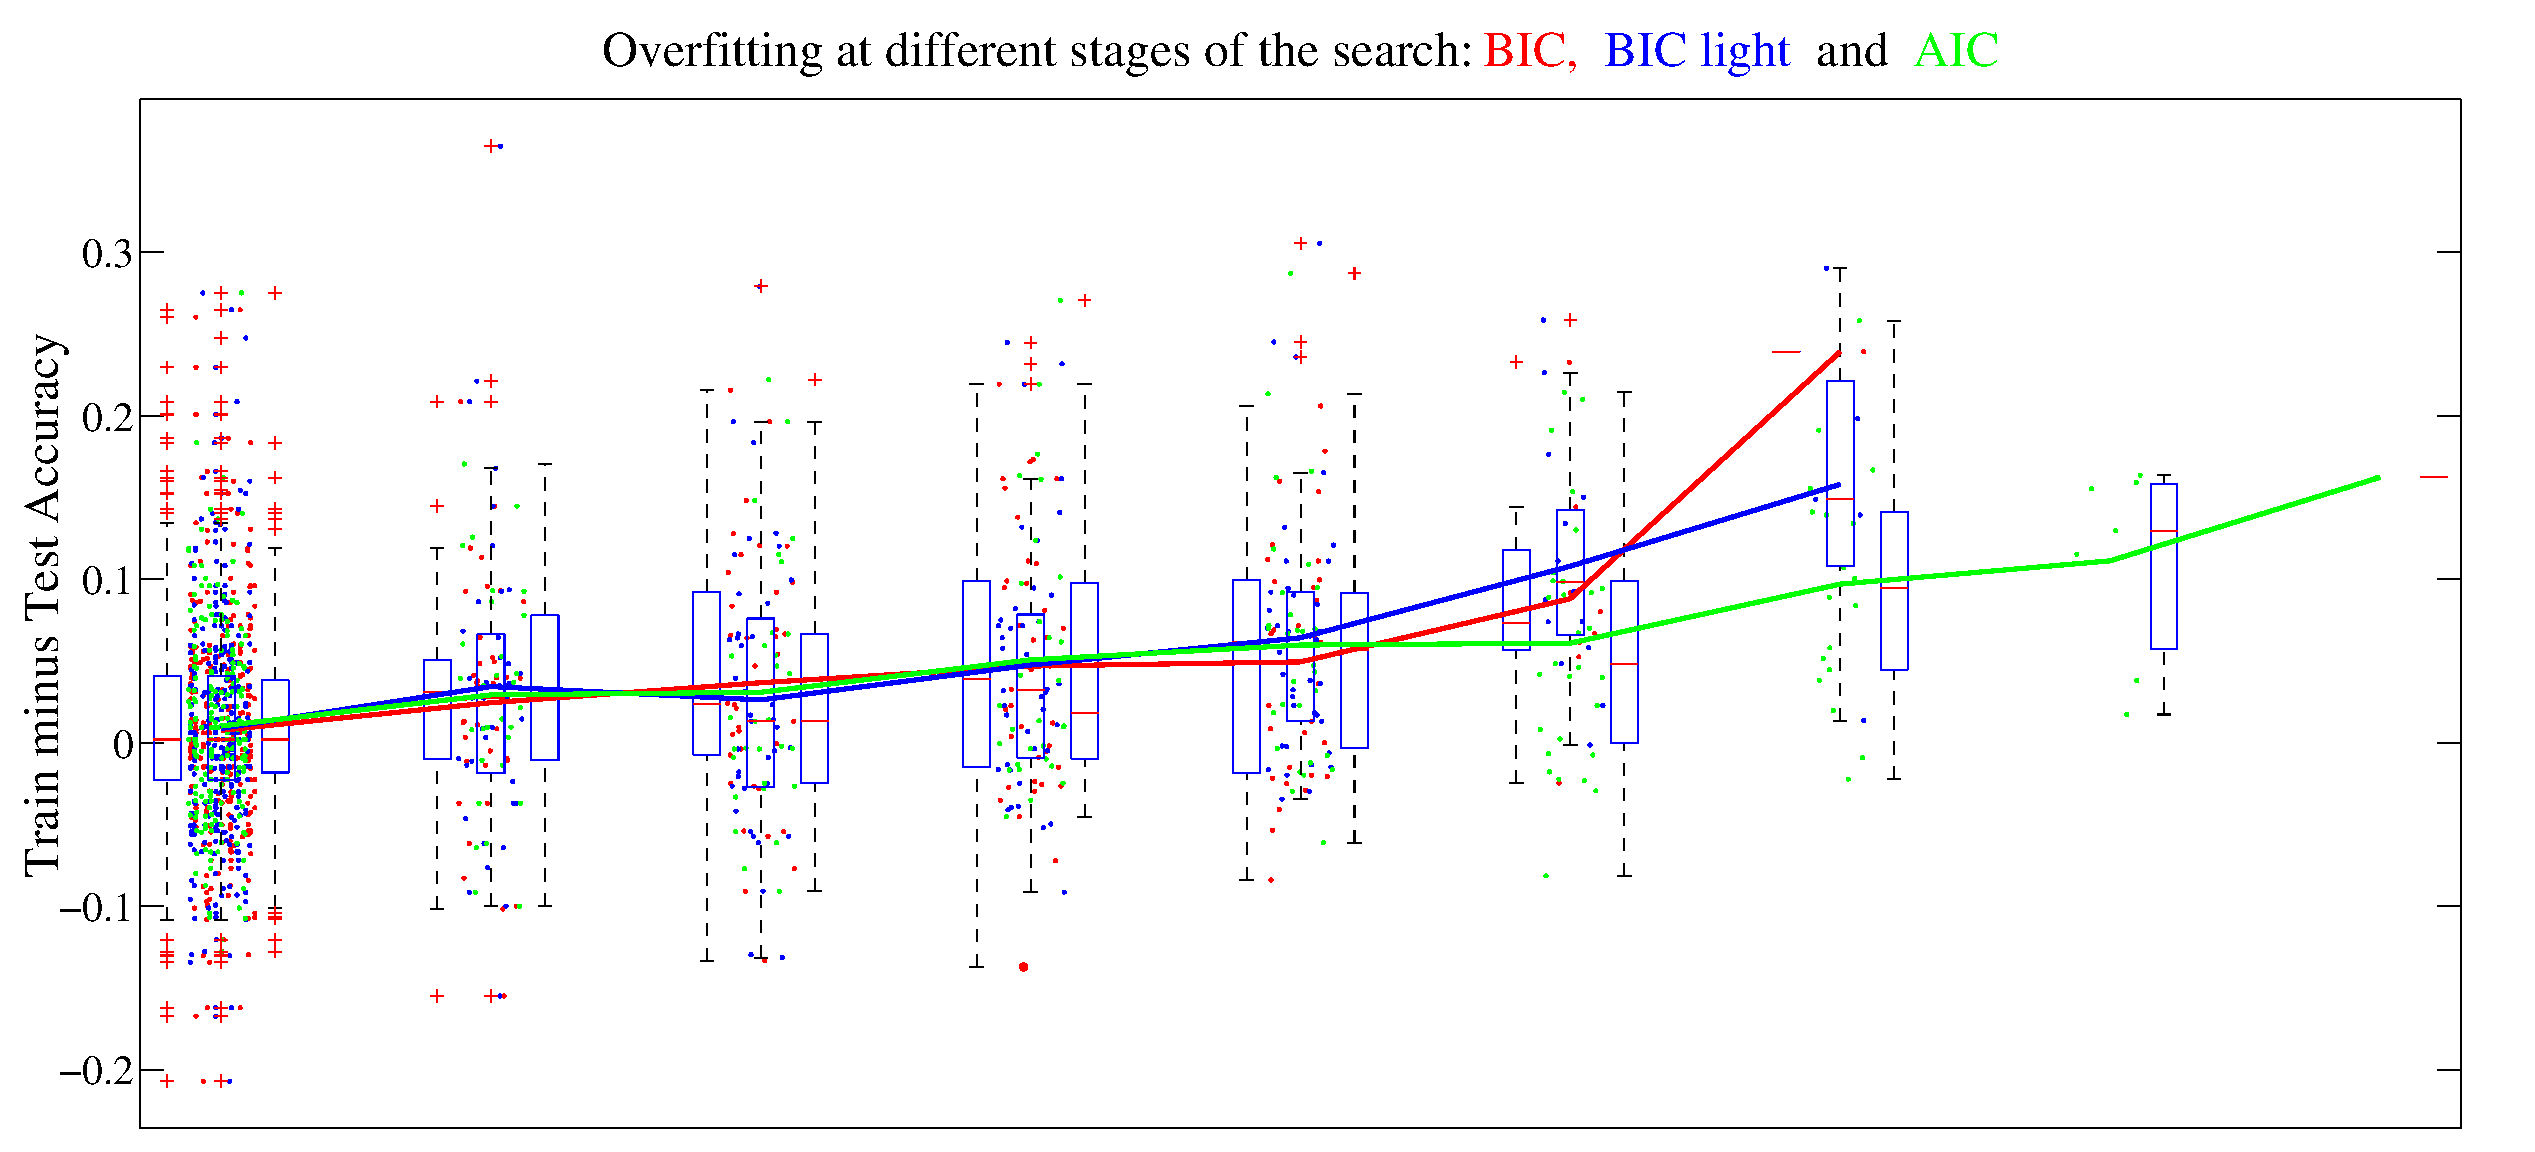
\includegraphics[trim=0cm 0cm 0cm 0cm, width=1\textwidth]{figures/overfitting}
\end{center}

\caption{The level of overfitting at each stage of the search, averaged over all experiments across the four data sets. The box plots show the 25th and 75th data percentile.}

\end{figure}


Figure 4.2 shows the levels of overfitting recorded across the search stages of all the experiments. The difference between train and test accuracies increases in the later stages of the search. For search stages with significant numbers of data points for all three criteria (up to depth five), the levels of overfitting are similar for all three methods. Due to different penalisation factors for model complexity, the BIC search stops first and the AIC search builds the most elaborate kernel structures.

Bayesian methods such as Gaussian Processes should not overfit to such an extent. If we can explain why this overfitting occurs, we may be able to improve the search procedure in order to minimise it. If not, we will at least understand the fundamental limitations of this approach.


%The poor performance of the structure search in that example comes from overfitting, which happens because of the small size of the data set

% - Taking wrong turns vs bad lengthscales. ...  We will discuss in what ways the search can fail, and what the possible avenues for minimising such errors are.

\subsubsection*{Overfitting with Small Lengthscales}

Kernel structures with weak test performance often include base components with very short lengthscales. As the latent function of such kernels varies quickly, it can achieve good model fit for most data sets. Kernels with extremely small lengthscales treat each observation as independent, making the resulting model overfit. Such pathological lengthscales are usually chosen when the data set can not be explained by smooth functions drawn from {\SE} priors.

In our experiments, this anomaly occurred whenever data sets contained discretised features (gender, age, number of pregnancies, etc.). The posterior plot for one such feature of the Liver data set is shown in Figure 4.3. If we were to trust the predictions of this model, we could make some very interesting conclusions. For example, drinking two to three pints a day causes liver failure with absolute certainty. To avoid this fate, one should make sure to drink more (or less) than that. \\

%\includegraphics[width=1\textwidth] {figures/liversmalllengthscale.png}

\begin{figure} [!ht]
\caption{Overfitting using short lengthscales on the Liver data set. }
\begin{center}
\includegraphics[trim=0cm 0cm 0cm 0cm, width=1\textwidth]{figures/overfitsmall.eps}
\end{center}
\end{figure}

Overfitting of this type can be avoided using relatively simple heuristics. For input dimensions with discretised features, the minimal lengthscale used should not be shorter than the minimal distance between non-unique values of this feature. Removing the kernels which violate this condition from the search space ensured that the procedure could no longer overfit using short lengthscales. Discretised features remain problematic, as finding interpretable components for these dimensions is possible only in the simplest scenarios. However, this is a weakness of the kernel grammar, and not the search procedure itself.

\subsubsection*{Overfitting due to Small Sample Size}

Solving the problem of short lengthscales still left us with a number of experiments with large differences between train and test accuracies, even though the kernels constructed used reasonable lengthscales across all dimensions.

The mean accuracy is computed using ten-fold cross validation, and weak mean performance is usually attributable to folds with particularly bad test accuracies. The Liver data set contains 345 examples, which means that the test set contains around 35 examples on average. With such small sample sizes, the variance of the test accuracy across different folds becomes very large.

To get a sense of the variance in the accuracies, we identified the best-performing kernel structure across our experiments on the Liver data set. We optimised the hyperparameters of this model using the entire data set, and then applied it to 100 different ten fold cross-validation data splits. This means that we used our already trained model to compute the train and test set accuracies for 1000 different folds.

% $\SE_1 \kernplus \SE_3 \kerntimes \SE_4 \kerntimes \SE_5 \kernplus \SE_6$

\begin{figure} [ht!]
\caption{Train and test accuracies across 100 ten-fold cross validation experiments. }
\begin{center}
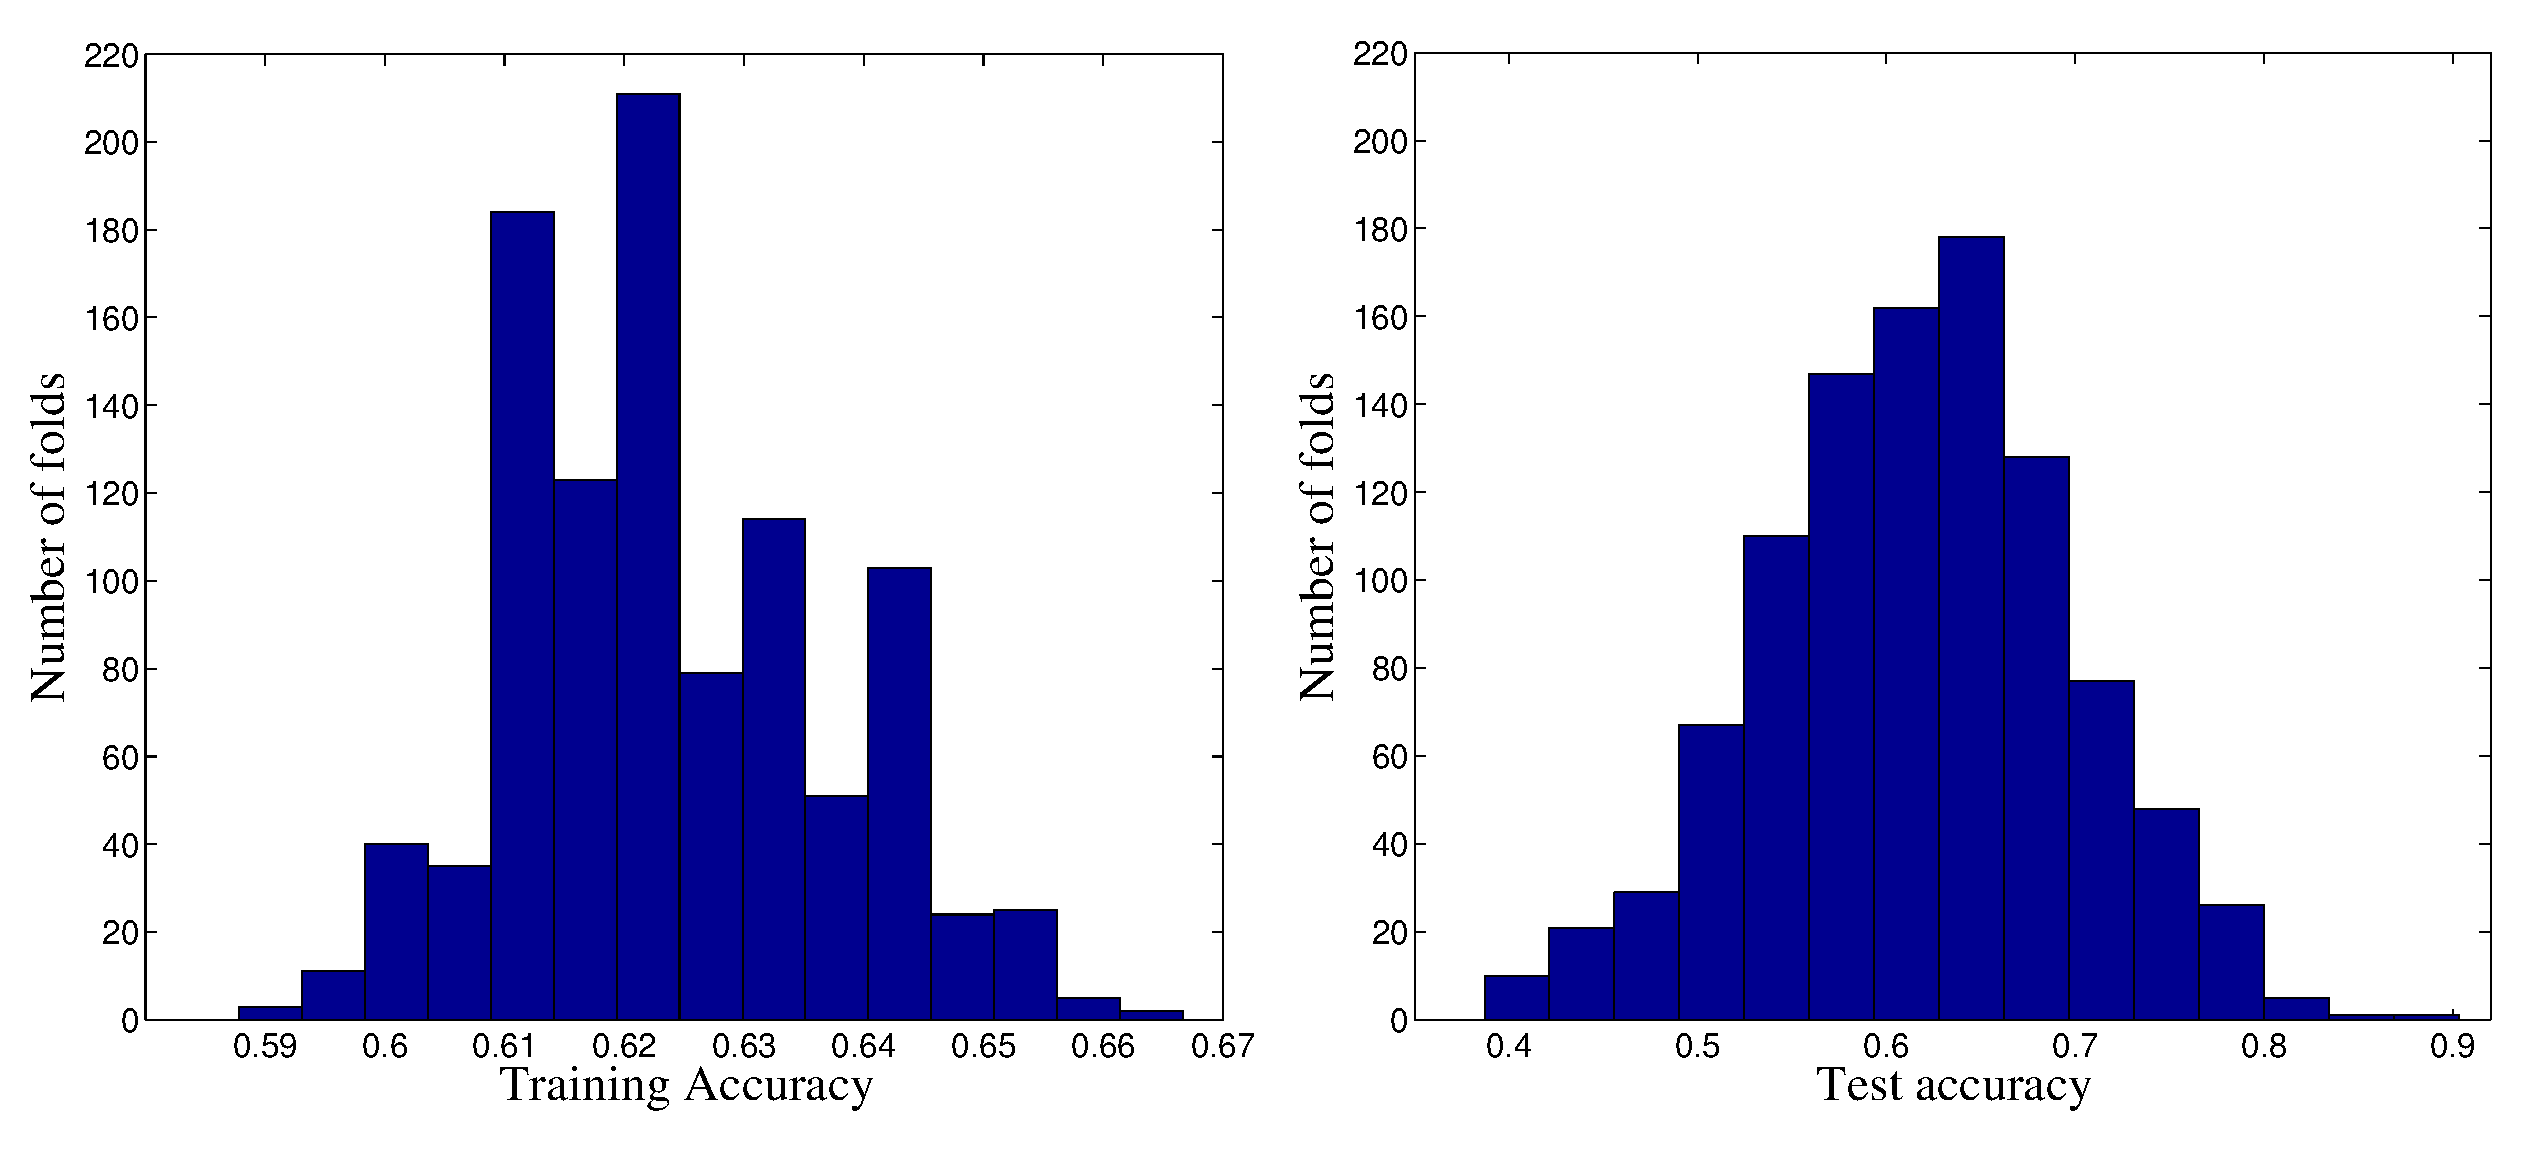
\includegraphics[trim=0cm 0cm 0cm 0cm, width=1\textwidth] {figures/overfitwithlargelength.eps}
\end{center}
\end{figure}


The histogram of the train and test set accuracies achieved across all the folds in these experiments is shown in Figure 4.4. Across the 1000 train-test splits produced, the training accuracy ranged from $59\%$ to $66\%$, while the test set accuracy varied from $40\%$ to $90\%$. This is somewhat surprising, as the model hyperparameters were trained using the entire data set.

This experiment confirms that the use of relatively small data sets (such as Liver) for ten-fold cross validation introduces a lot of variance into the test accuracy estimate. We were unable to find any structural problems with the kernel structures which exhibited bad test performance. On the contrary, these models performed well given different test sets, leading us to conclude that the weak test accuracies on some folds are not caused by issues related to overfitting or model misspecification.

\section{Providing Interpretability}

% In this section, we show how the models constructed by our procedure can be used to analyse data sets and draw conclusions about the problems these data sets deal with.

The additive components of the kernel structures chosen by the search can reveal important dependencies and patterns in the data sets. The most natural way to represent these patterns is to visualise the posterior means of the additive components. The classification boundaries given by these means can be used to draw conclusions about the problems that the data sets deal with. In this section, we show how the plots that our procedure creates for the Pima and Breast data sets can be used to draw conclusions about the underlying problems: predicting the occurrences of diabetes and breast cancer.

In our experiments, we used ten-fold cross validation to obtain an estimate of the procedure's test accuracy. As explained in the previous section, there is a lot of variability in the results obtained across different folds. The kernel structures identified vary across the folds, even though around 90\% of the examples are shared between any two folds' training data sets. The ten structures identified usually involve similar base kernels, but combine them into different expressions. For each data set, we address those kernel structures which were identified the most frequently.


% The remaining four attributes seem to carry less information regarding the likelihood of developing diabetes, at least in a dataset of this size and using this search procedure. These four features are the number of pregnancies, diastolic blood pressure, triceps skin fold thickness and 2-hour serum insulin measures.

\subsection{Pima Indian Diabetes Dataset}

The Pima Indian Diabetes dataset contains medical measurements of 768 individuals, together with an indicator of whether they later developed diabetes or not. The four most prominent base kernels across the kernel structures produced for the ten folds were $\SE_2, \SE_6, \SE_7$ and $\SE_8$. These represent the plasma glucose concentration, body mass index (BMI), diabetes pedigree function and the age of the patient. We will analyse the decompositions of the two kernel structures most frequently recovered.

\begin{figure}

\caption{The posterior mean plots of the additive components of $\SE_2\kerntimes\SE_7 \kernplus \SE_6 \kernplus \SE_8$. This kernel structure was identified in four out of ten cross validation experiments on the Pima data set. }

\begin{center}

\includegraphics[trim=0cm 0cm 0cm 0cm, width=0.9\textwidth]{figures/pima/age.png} % 8
\includegraphics[trim=0cm 0cm 0cm 0cm, width=0.9\textwidth]{figures/pima/bmi.png} % 6
\includegraphics[trim=0cm 0cm 0cm 0cm, width=0.9\textwidth]{figures/pima/pedigreeglucose.png}  % 2 x 7

\end{center}

\end{figure}


\begin{figure}

\caption{The posterior mean plots of the additive components of $\SE_2 \kernplus \SE_6 \times \SE_7 \kernplus \SE_8$. This kernel structure was identified in three out of ten cross validation experiments on the Pima data set.}

\begin{center}

\includegraphics[trim=0cm 0cm 0cm 0cm, width=0.9\textwidth]{figures/pima/age.png} % 8
\includegraphics[trim=0cm 0cm 0cm 0cm, width=0.9\textwidth]{figures/pima/glucose.png} % 2
\includegraphics[trim=0cm 0cm 0cm 0cm, width=0.9\textwidth]{figures/pima/pedigreebmi.png} % 6 x 7

\end{center}

\end{figure}

The decomposition of $\SE_2\kerntimes\SE_7 \kernplus \SE_6 \kernplus \SE_8$ (identified in four folds) is shown in Figure 4.5. The first component indicates that those between the ages of 27 and 60 are more likely to be diagnosed with diabetes than those who are younger or older. Dependencies such as this one are not expressible using simpler models such as logistic regression. The second component shows that diabetes occurrence correlates with the body mass index: anyone with a BMI of over 30 is at (high) risk of being diagnosed. The third component shows the two-way interaction between the diabetes pedigree function (the genetic likelihood of getting diabetes) and the plasma glucose concentration. This plot is hard to interpret: the classification boundary indicates that the high glucose concentration is a better indicator of diabetes occurrence for people with a high pedigree function. This trend is not particularly obvious in the data points.

Figure 4.6 shows the decomposition of $ \SE_2 \kernplus \SE_6 \times \SE_7 \kernplus \SE_8$, identified in three different folds. The age dependency is still present, and the glucose concentration becomes a one-dimensional component: as expected, the higher it is, the more likely the person is to become diabetic. The third component is a two-way interaction between diabetes pedigree and the BMI. This plot achieves great data separation, and leads to an interesting conclusion: people with a history of diabetes in the family can avoid it by staying in shape, whereas those without a history of diabetes are still at risk if they are overly obese (as shown by the two peaks in the contours representing the regions of high risk).


%Another structure frequently identified was $ 2 \kernplus 6 \times 7 \kernplus 8$. The plot of the new component, showing the dependency between the BMI and the diabetes pedigree function is given by:

\subsection{Wisconsin Diagnostic Breast Cancer Dataset}

Wisconsin Diagnostic Breast Cancer Dataset is a nine-dimensional dataset which contains measured attributes of 449 individuals, together with an indicator of whether or not they later developed breast cancer. The base kernels most frequently used in the structures identified were $\SE_1, \SE_2, \SE_4, \SE_6$ and $\SE_8$. Most of the kernel structures identified include three-way interactions: $\SE_1 \kerntimes \SE_2 \kerntimes \SE_6$ appears in three folds, as do some other high dimensional interactions. Unfortunately, our procedure is still unable to visualise the high-dimensional components.

Figure 4.7 contains the one-dimensional components of the kernel structure given by $ \SE_1 \kernplus  \SE_2 \kerntimes \SE_6 \kerntimes \SE_8 \kernplus \SE_5 $. $\SE_5$ represents the patients' epithelial cell size, and $\SE_1$ represents the measured clump thickness. Both components' means have a clear cut-off value, after which patients are predicted to get breast cancer. The posterior mean of the first component (epithelial cell size) is interesting: linear models could not express such a dependency. The third component of the kernel is given by a three way interaction, which we are still unable to visualise. \\

\begin{figure} [h]

\caption{The posterior mean plots of the one-dimensional additive components of $\SE_1 \kernplus  \SE_2 \kerntimes \SE_6 \kerntimes \SE_8 \kernplus \SE_5 $, identified in the Breast data set experiments.}

\begin{center}

%\makebox[(\textwidth) ]{

\includegraphics[trim=1.5cm 0cm 1.5cm 0cm, width=0.65\textwidth]{figures/breast/cellsize.png} % 5
\includegraphics[trim=1.5cm 0cm 1.5cm 0cm, width=0.65\textwidth]{figures/breast/clump.png} % 1

%}

\end{center}


\end{figure}



The kernel structure $\SE_1 \kerntimes \SE_7 \kernplus \SE_2 \kerntimes \SE_6 $ is the only identified structure for which we can currently visualise all the additive components. The plots in Figure 4.8 show these two-way interactions: the classification boundaries given by both of their posterior means separate the data well, as is to be expected given that the test accuracy on this fold was 95.45\%.

The dependence between dimensions in these two plots is not very pronounced: these kernel products could have been represented as sums of two base kernels. Whether we choose the sum or the product depends on the models' approximate marginal likelihoods. As these estimates are sensitive to changes in the training data, we identify many different kernel structures across the ten folds. \\

\begin{figure} [h]

\caption{The posterior mean plots of the two additive components in the kernel structure: $ \SE_2 \kerntimes \SE_6 \kernplus \SE_7 \kerntimes \SE_1 $, identified in the Breast data set experiments.}

\begin{center}

\includegraphics[trim=0cm 0cm 0cm 0cm, width=0.95\textwidth]{figures/breast/nucleicellsize.png} % 7 x 1
\includegraphics[trim=0cm 0cm 0cm 0cm, width=0.95\textwidth]{figures/breast/clumpbland.png} % 2 x 6

\end{center}

\end{figure}

\cleardoublepage

\chapter{Towards the Automated Statistician}

In this chapter, we investigate how the implemented kernel discovery procedure can be used to move towards our long term goal of creating an automated statistician for classification. We will analyse how our approach can be extended to:

\begin{enumerate}

\item {Create robust classifiers:} the discovery procedure can be extended to learn data set specific likelihood functions which make the constructed models less susceptible to outliers in the data.

\item {Maximise predictive performance:} combining the predictions made by all the models evaluated at different stages of the search reduces the risk of choosing weak models and allows us to make better predictions.

\end{enumerate}

\section{Robust Gaussian Process Classification}

In classification data sets, most of the noise in the class labels comes from mislabelled examples which lie close to the classification boundary. The class membership of points in this region is often ambiguous, making it hard to classify these examples consistently \cite{kim08}. The rest of the noise comes from \emph{complete outliers}, that is labelling errors far from the classification boundary. Outliers are usually the product of errors in the examples' input space, such as wrong measurements of the feature values. We will refer to these labelling errors as the \emph{salt and pepper noise}.

An aspect important for the applicability of classification models to real-world data sets is their ability to deal with this type of noise. Classification specific methods such as soft-margin support vector machines have been designed with the existence of outliers in mind. These models are less certain of their predictions, as the soft margin parameter allows for a certain proportion of each classes' examples to be left on the wrong side of the separating hyperplane. Standard GP classifiers assume there is no noise in the input space: likelihood models such as the cumulative Gaussian (error) function can only handle noise in the output space, that is misclassified examples which were somewhat ambiguous to begin with.

GP classification models produce probabilistic predictions, which means that they inform the user of the level of certainty about the predictions made. This is one of the appealing features of GPs, but it also means that these models tend to be very certain about the class membership of points in high density regions which lie far from the classification boundary. For this reason, it becomes very hard to learn good models for training data sets which contain salt and pepper noise.

\subsection{Modifying the Likelihood Function}

To address this issue, we add another dimension to the GP structure search. In addition to learning the kernel structure, the procedure will also adapt the likelihood function so that the model built becomes less susceptible to complete outliers in the data. The error function likelihood is replaced by a linear mixture of two likelihood functions: the error function itself and a uniform likelihood function.

The uniform likelihood acts as the noise model for the outliers: their class membership is treated as being completely random.  The {salt and pepper} noise level $\epsilon$ refers to the proportion of complete outliers in the data set. This value determines the weight to be assigned to the uniform likelihood function in the likelihood mixture.

The probabilistic predictions of this model no longer range from 0 to 1, but from $\frac{\epsilon}{2}$ to $1 - \frac{\epsilon}{2}$, reflecting the uncertainty in predictions due to the outliers present in the data set. Likelihood functions for different mixture rates are shown in Figure 5.1.

\begin{figure}
\caption{Mixtures of likelihood functions for different levels of salt and pepper noise.}
\begin{center}
\includegraphics[trim=0cm 0cm 0cm 0cm, width=1\textwidth] {figures/likMixPlot.eps}
\end{center}
\end{figure}


The noise rate $\epsilon$ is a new hyperparameter of the model, to be estimated from the training data along with the kernel hyperparameters. If the structure search that builds models which use this likelihood function has the potential to improve performance on noisy data sets, it should be capable of correctly estimating the proportion of outliers in them.





\subsection{Evaluating the Likelihood Mixture Model}

% we drew the latent function from their \gp{} priors. We then added \iid Gaussian noise with different SNR ratios, as well as different amounts of \emph{salt and pepper noise}. The SP noise represents the random outliers: we add these into the synthetic data set by flipping the labels of a random sub-sample of its examples.


In this section, we analyse the results achieved by the BIC light guided structure search which builds GP models using the proposed likelihood function. As the GPML toolbox supports likelihood mixtures, we were able to extend our structure search implementation to this new family of models. The procedure was then applied to four synthetic data sets drawn from GP priors, as well as the four real-world data sets previously considered.

%The ability of the new model to recover known structures was evaluated on synthetic data sets drawn from four different composite kernels.

In these experiments, our first goal was to determine whether hyperparameter fitting based on optimising the marginal likelihood could estimate the noise level correctly. If so, we wanted to determine how much (and if) the new models improve on the performance achieved by GP models which used the stand-alone error function as the likelihood model.

\subsubsection*{Experiments on Synthetic Data Sets}

Across the synthetic experiments, the noise level estimation failed for most data sets which contained salt and pepper noise. For noise-free data sets, the level of noise was estimated correctly. For the majority of the noisy data sets, the procedure either concluded that there was no noise or it vastly overestimated the noise level. The details and the full results of these experiments are given in Appendix B.

The more complex the kernel structure in an experiment is, the more likely the noise estimation is to fail. The results of the experiments on the synthetic data set drawn from the most complex kernel structure are summarised in Table 5.1. Whenever the noise level was overestimated, kernel discovery failed completely. The procedure returned arbitrary one-dimensional kernel structures whose test accuracies dropped to the baseline levels of around 50\% (see Appendix B).



\begin{table}[h]

\caption{{ True kernel: $ \SE_1 + \SE_2 + \SE_3$, $D$ = 3.           }}

\label{tbl:syntheticLik1}


\begin{center}
{\small
\makebox[\textwidth]{


\begin{tabular}{|c c  c | c |  c | c c| }
\hline Data size & SNR & sp\_noise &  Kernel chosen & Test accuracy & Kernel rate & Bayes rate \\

\hline
100& 100& 0\% & ${1} + {1} \times {3} + {2}$ &87.0\% & 91.0\% & 97.4\%   \\ 
300& 100& 0\% & ${1} + {2} + {3}$ &94.0\% & 95.7\% & 97.4\%    \\
500& 100& 0\% & ${1} + {2} + {3}$ &95.8\% & 95.4\% & 97.4\%  \\  \hline
100& 100& 5\% & ${1} + {2} + {3}$ &77.0\% & 80.0\% & 91.6\%    \\
300& 100& 5\% & ${1} \times {3} + {2}$ &87.0\% & 85.7\% & 91.6\%  \\    
500& 100& 5\% & ${1} \times {2} \times {3}$ &89.8\% & 89.8\% & 91.6\%   \\  \hline
100& 100& 20\% & ${1} \times {3}$ &69.0\% & 69.0\% & 82.0\%    \\
300& 100& 20\% & ${1} \times {3} + {2}$ &75.3\% & 73.0\% & 82.0\%    \\
500& 100& 20\% & ${1} \times {3} + {2}$ &77.6\% & 74.0\% & 82.0\%   \\ \hline
100& 1& 0\% & ${1} + {3}$ &64.0\% & 72.0\% & 77.4\%    \\
300& 1& 0\% & ${1} + {3}$ &74.3\% & 75.0\% & 77.4\%    \\
500& 1& 0\% & ${1} + {3}$ &75.6\% & 76.6\% & 77.4\%  \\  \hline
100& 1& 5\% & ${1} + {3}$ &63.0\% & 63.0\% & 74.4\%    \\
300& 1& 5\% & ${1} \times {3}$ &70.7\% & 68.3\% &  74.4\%    \\
500& 1& 5\% & ${1} \times {3}$ &72.6\% & 72.6\% & 74.4\%  \\  \hline
100& 1& 20\% & ${1} \times {3}$ &53.0\% & 60.0\% & 68.8\%    \\
300& 1& 20\% & ${1} \times {3}$ &65.3\% & 65.3\% & 68.8\%    \\
500& 1& 20\% & ${1} \times {3}$ &66.2\% & 67.8\% & 68.8\%   \\
\hline

\end{tabular}
} }
\end{center}


\end{table}


\begin{table}[h]

\caption{{ True kernel: $ \SE_1 + \SE_2 + \SE_3$, $D$ = 3.           }}

\label{tbl:syntheticlik2}


\begin{center}
{\small
\makebox[\textwidth]{


\begin{tabular}{|c c  c | c |  c | c c| c | }
\hline Data size & SNR & sp\_noise &  Kernel chosen & Test accuracy & Kernel rate & Bayes rate & Noise ratio \\

\hline
100& 	100& 	0\% & 	${1} \times {3}$ &	92.0\% & 	91.0\% & 	97.4\%    	 &  0.0\%  \\ 
300& 	100& 	0\% & 	${1} + {2} + {3}$ &	94.0\% & 	95.7\% & 	97.4\%    	 &  0.0\%  \\ 
500& 	100& 	0\% & 	${1} \times {3} + {2} + {3}$ &	94.8\% & 	95.4\% & 	97.4\%    	 &  0.0\%  \\  \hline
100& 	100& 	5\% & 	${1} + {3}$ &	80.0\% & 	79.0\% & 	91.6\%    	 &  0.0\%  \\ 
300& 	100& 	5\% & 	${1} + {1} \times {3} + {2}$ &	87.0\% & 	89.3\% & 	91.6\%    	 &  11.8\%  \\ 
500& 	100& 	5\% & 	${1} \times {3} + {2} + {2} \times {2}$ &	89.2\% & 	90.6\% & 	91.6\%    	 &  13.9\%  \\  \hline
100& 	100& 	20\% & 	${1} \times {3}$ &	69.0\% & 	64.0\% & 	82.0\%    	 &  0.0\%  \\ 
300& 	100& 	20\% & 	${1} \times {3}$ &	75.0\% & 	74.7\% & 	82.0\%    	 &  32.2\%  \\ 
500& 	100& 	20\% & 	${1} \times {3} + {2}$ &	77.2\% & 	75.0\% & 	82.0\%    	 &  33.3\%  \\   \hline
100& 	1& 	0\% & 	${1} + {3}$ &	64.0\% & 	71.0\% & 	77.4\%    	 &  0.0\%  \\ 
300& 	1& 	0\% & 	${1} + {3}$ &	74.0\% & 	73.7\% & 	77.4\%    	 &  5.3\%  \\ 
500& 	1& 	0\% & 	${1} + {3}$ &	76.0\% & 	76.4\% & 	77.4\%    	 &  0.0\%  \\  \hline
100& 	1& 	5\% & 	${1} + {3}$ &	63.0\% & 	63.0\% & 	74.4\%    	 &  0.0\%  \\ 
300& 	1& 	5\% & 	${1} + {3}$ &	72.0\% & 	71.0\% & 	74.4\%    	 &  12.9\%  \\ 
500& 	1& 	5\% & 	${1} \times {3}$ &	72.6\% & 	73.2\% & 	74.4\%    	 &  0.0\%  \\  \hline
100& 	1& 	20\% & 	${1} \times {3}$ &	53.0\% & 	61.0\% & 	68.8\%    	 &  0.0\%  \\ 
300& 	1& 	20\% & 	${1} \times {3}$ &	65.3\% & 	65.7\% & 	68.8\%    	 &  0.1\%  \\ 
500& 	1& 	20\% & 	${1} \times {3}$ &	68.0\% & 	67.6\% & 	68.8\%    	 &  0.3\%  \\ 

\hline

\end{tabular}
} }
\end{center}


\end{table}







\begin{table*}[h]
\caption{{ True kernel: $ \SE_1 + \SE_2 \times \SE_3 + \SE_4$,  $D$ = 4.           }}
 

\label{tbl:synthetic3}
\begin{center}
{\small
\makebox[\textwidth]{
\begin{tabular}{|c c  c | c |  c | c c| }
\hline Data size & SNR & sp\_noise &  Kernel chosen & Test accuracy & Kernel rate & Bayes rate \\

\hline
100& 100& 0\% & ${1} + {2} \times {3} + {4}$ &87.0\% & 92.0\% & 97.4\%    \\
300& 100& 0\% & ${1} + {2} \times {3} + {4}$ &94.0\% & 94.7\% & 97.4\%    \\
500& 100& 0\% & ${1} + {2} \times {3} + {4}$ &95.6\% & 96.2\% & 97.4\%    \\  \hline
100& 100& 5\% & ${1} + {2}$ &81.0\% & 76.0\% & 92.0\%    \\
300& 100& 5\% & ${1} + {2} + {3} \times {4}$ &85.7\% & 84.0\% & 92.0\%     \\
500& 100& 5\% & ${1} \times {4} + {2} \times {3} + {3}$ &87.6\% & 88.6\% & 92.0\%  \\  \hline
100& 100& 20\% & ${2} \times {4}$ &67.0\% & 67.0\% & 82.0\%    \\
300& 100& 20\% & ${2} \times {3} + {4}$ &76.0\% & 73.7\% & 82.0\%    \\
500& 100& 20\% & ${2} + {3} \times {4}$ &77.0\% & 79.8\% & 82.0\%   \\ \hline
100& 1& 0\% & ${2}$ &68.0\% & 67.0\% & 76.0\%    \\
300& 1& 0\% & ${1} + {2} \times {3}$ &72.3\% & 70.3\% & 76.0\%    \\
500& 1& 0\% & ${1} + {2} \times {3}$ &72.2\% & 73.2\% & 76.0\%  \\  \hline
100& 1& 5\% & ${2}$ &67.0\% & 58.0\% & 72.2\%    \\
300& 1& 5\% & ${1} \times {2}$ &71.0\% & 64.3\% & 72.2\%    \\
500& 1& 5\% & ${1} \times {2} \times {3}$ &70.6\% & 68.0\% & 72.2\%  \\  \hline
100& 1& 20\% & ${2}$ &59.0\% & 61.0\% & 69.0\%    \\
300& 1& 20\% & ${2} \times {3} \times {4}$ &65.3\% & 62.3\% & 69.0\%    \\
500& 1& 20\% & ${2} \times {3} \times {4}$ &64.8\% & 64.8\% & 69.0\%    \\

\hline
\end{tabular}
} }
\end{center}
\end{table*}


\begin{table}[h]

\caption{{ True kernel: $ \SE_1 + \SE_2 \times \SE_3 + \SE_4$,  $D$ = 4.          }}

\label{tbl:syntheticLik4}


\begin{center}
{\small
\makebox[\textwidth]{


\begin{tabular}{|c c  c | c |  c | c c| c | }
\hline Data size & SNR & sp\_noise &  Kernel chosen & Test accuracy & Kernel rate & Bayes rate & Noise ratio \\

\hline
100& 	100& 	0\% & 	${1} + {2} \times {3} + {4}$ &	87.0\% & 	92.0\% & 	97.4\%    	 &  0.0\%  \\ 
300& 	100& 	0\% & 	${1} + {2} \times {3} + {4}$ &	94.0\% & 	94.7\% & 	97.4\%    	 &  0.0\%  \\ 
500& 	100& 	0\% & 	${1} + {2} \times {3} + {4}$ &	95.4\% & 	96.2\% & 	97.4\%    	 &  0.0\%  \\ \hline
100& 	100& 	5\% & 	${1} \times {2} + {2}$ &	81.0\% & 	78.0\% & 	92.0\%    	 &  0.0\%  \\ 
300& 	100& 	5\% & 	${1} + {2} \times {3} + {4}$ &	87.3\% & 	88.3\% & 	92.0\%    	 &  9.9\%  \\ 
500& 	100& 	5\% & 	${1} + {2} \times {3} + {3} + {4}$ &	90.2\% & 	89.6\% & 	92.0\%    	 &  12.8\%  \\ \hline
100& 	100& 	20\% & 	${1} \times {4} + {2}$ &	64.0\% & 	65.0\% & 	82.0\%    	 &  18.8\%  \\ 
300& 	100& 	20\% & 	${2} \times {3} + {4}$ &	75.7\% & 	74.3\% & 	82.0\%    	 &  9.4\%  \\ 
500& 	100& 	20\% & 	${1} \times {3} + {2} + {4}$ &	77.0\% & 	78.8\% & 	82.0\%    	 &  30.5\%  \\ \hline
100& 	1& 	0\% & 	${2}$ &	69.0\% & 	65.0\% & 	76.0\%    	 &  54.4\%  \\ 
300& 	1& 	0\% & 	${1} + {2} \times {3}$ &	72.3\% & 	73.0\% & 	76.0\%    	 &  0.0\%  \\ 
500& 	1& 	0\% & 	${1} + {2} \times {3} + {4}$ &	72.2\% & 	73.2\% & 	76.0\%    	 &  0.0\%  \\ \hline
100& 	1& 	5\% & 	${2}$ &	67.0\% & 	58.0\% & 	72.2\%    	 &  43.1\%  \\ 
300& 	1& 	5\% & 	${1} \times {2}$ &	71.0\% & 	65.0\% & 	72.2\%    	 &  2.6\%  \\ 
500& 	1& 	5\% & 	${1} \times {2} + {3}$ &	70.2\% & 	68.8\% & 	72.2\%    	 &  29.0\%  \\ \hline
100& 	1& 	20\% & 	${2}$ &	59.0\% & 	63.0\% & 	69.0\%    	 &  40.6\%  \\ 
300& 	1& 	20\% & 	${2}$ &	63.3\% & 	60.7\% & 	69.0\%    	 &  51.3\%  \\ 
500& 	1& 	20\% & 	${2} \times {3}$ &	63.4\% & 	64.2\% & 	69.0\%    	 &  57.6\%  \\ 

\hline

\end{tabular}
} }
\end{center}


\end{table}





\begin{table*}[h]
\caption{{True kernel: $ \SE_1 + \SE_3 \times \SE_7 + \SE_{10}$,  $D$ = 10.  }} 

\label{tbl:syntheticlik5}
\begin{center}
{\small

\makebox[\textwidth]{

\begin{tabular}{|c c  c | c |  c | c c| }
\hline Data size & SNR & sp\_noise &  Kernel chosen & Test accuracy & Kernel rate & Bayes rate \\

\hline
100& 100& 0\% & ${1} \times {9} + {10}$ &61.0\% & 88.0\% & 96.0\%    \\
300& 100& 0\% & ${1} + {1} \times {10} + {3} \times {7}$ &92.0\% & 92.7\% & 96.0\%    \\
500& 100& 0\% & ${1} + {1} \times {3} \times {7} \times {10} + {10}$ &94.2\% & 94.6\% & 96.0\%   \\ \hline
100& 100& 5\% & ${1} \times {9} + {10}$ &53.0\% & 71.0\% & 91.8\%    \\
300& 100& 5\% & ${1} + {3} \times {7} + {6} \times {10}$ &82.0\% & 81.3\% & 91.8\%    \\
500& 100& 5\% & ${1} \times {3} \times {7} \times {10} + {10}$ &85.0\% & 86.2\% & 91.8\%   \\ \hline
100& 100& 20\% & ${1}$ &49.0\% & 64.0\% & 79.8\%    \\
300& 100& 20\% & ${1} + {10}$ &60.0\% & 70.0\% & 79.8\%    \\
500& 100& 20\% & ${1} \times {3} \times {7} \times {10}$ &74.2\% & 75.2\% & 79.8\%   \\ \hline
100& 1& 0\% & ${10}$ &59.0\% & 70.0\% & 74.4\%    \\
300& 1& 0\% & ${1} \times {3} \times {7} \times {10} + {10}$ &71.3\% & 72.7\% & 74.4\%    \\
500& 1& 0\% & ${1} \times {10} + {3} \times {7} + {9}$ & 72.0\% & 71.4\% & 74.4\%   \\ \hline
100& 1& 5\% & ${10}$ &55.0\% & 66.0\% & 71.4\%    \\
300& 1& 5\% & ${1} \times {10}$ &58.7\% & 68.7\% & 71.4\%    \\
500& 1& 5\% & ${1} + {10}$ &60.6\% & 69.4\% & 71.4\%  \\  \hline
100& 1& 20\% & ${3}$ &55.0\% & 56.0\% & 65.4\%    \\
300& 1& 20\% & ${10}$ &58.0\% & 61.7\% & 65.4\%    \\
500& 1& 20\% & ${1} \times {10}$ &58.2\% & 62.0\% & 65.4\%    \\
 

\hline
\end{tabular}
} }
\end{center}
\end{table*}

\begin{table}[h]

\caption{{ True kernel: $ \SE_1 + \SE_3 \times \SE_7 + \SE_{10}$,  $D$ = 10.         }}

\label{tbl:syntheticlik6}


\begin{center}
{\small
\makebox[\textwidth]{


\begin{tabular}{|c c  c | c |  c | c c| c | }
\hline Data size & SNR & sp\_noise &  Kernel chosen & Test accuracy & Kernel rate & Bayes rate & Noise ratio \\

\hline

100& 	100& 	0\% & 	${10}$ &	62.0\% & 	88.0\% & 	96.0\%    	 &  20.4\%  \\ 
300& 	100& 	0\% & 	${1} + {3} \times {7} + {10}$ &	92.0\% & 	93.0\% & 	96.0\%    	 &  0.0\%  \\ 
500& 	100& 	0\% & 	${1} \times {7} \times {10}$ &	75.0\% & 	94.6\% & 	96.0\%    	 &  5.4\%  \\ \hline
100& 	100& 	5\% & 	${1} \times {9} + {10}$ &	53.0\% & 	75.0\% & 	91.8\%    	 &  0.0\%  \\ 
300& 	100& 	5\% & 	${1} + {3} \times {7} + {10}$ &	84.7\% & 	86.7\% & 	91.8\%    	 &  7.0\%  \\ 
500& 	100& 	5\% & 	${1} \times {10} + {3} \times {7}$ &	87.8\% & 	89.2\% & 	91.8\%    	 &  11.3\%  \\ \hline
100& 	100& 	20\% & 	${1}$ &	50.0\% & 	64.0\% & 	79.8\%    	 &  49.5\%  \\ 
300& 	100& 	20\% & 	${1} + {10}$ &	58.3\% & 	72.7\% & 	79.8\%    	 &  55.1\%  \\ 
500& 	100& 	20\% & 	${1} + {3} \times {7} + {10}$ &	77.2\% & 	77.4\% & 	79.8\%    	 &  28.2\%  \\ \hline
100& 	1& 	0\% & 	${10}$ &	58.0\% & 	73.0\% & 	74.4\%    	 &  6.9\%  \\ 
300& 	1& 	0\% & 	${1} \times {3} \times {7} \times {10} + {10}$ &	71.3\% & 	72.7\% & 	74.4\%    	 &  0.0\%  \\ 
500& 	1& 	0\% & 	${6}$ &	48.2\% & 	72.4\% & 	74.4\%    	 &  90.3\%  \\ \hline
100& 	1& 	5\% & 	${10}$ &	55.0\% & 	67.0\% & 	71.4\%    	 &  1.4\%  \\ 
300& 	1& 	5\% & 	${1} \times {10}$ &	58.7\% & 	69.0\% & 	71.4\%    	 &  0.0\%  \\ 
500& 	1& 	5\% & 	${10}$ &	57.2\% & 	70.4\% & 	71.4\%    	 &  74.2\%  \\ \hline
100& 	1& 	20\% & 	${10}$ &	62.0\% & 	57.0\% & 	65.4\%    	 &  53.0\%  \\ 
300& 	1& 	20\% & 	${10}$ &	58.0\% & 	62.7\% & 	65.4\%    	 &  0.2\%  \\ 
500& 	1& 	20\% & 	${10}$ &	58.8\% & 	62.8\% & 	65.4\%    	 &  0.1\%  \\ 

\hline

\end{tabular}
} }
\end{center}

\end{table}







 
 \begin{table*}[h]
\caption{{ True kernel: $\SE_1 + \SE_3 \times \SE_5 \times \SE_7 + \SE_{9}$,  $D$ = 10. }} 

\label{tbl:syntheticlik7}
\begin{center}
{\small

\makebox[\textwidth]{%

\begin{tabular}{|c c  c | c |  c | c c| }
\hline Data size & SNR & sp\_noise &  Kernel chosen & Test accuracy & Kernel rate & Bayes rate \\
\hline


100& 100& 0\% & ${3} \times {5} \times {7}$ &85.0\% & 86.0\% & 97.0\%    \\
300& 100& 0\% & ${3} \times {5} \times {7} + {9}$ &93.7\% & 93.0\% & 97.0\%    \\
500& 100& 0\% & ${3} \times {5} \times {7}$ &91.4\% & 92.2\% & 97.0\%   \\ \hline
100& 100& 5\% & ${3} \times {5} \times {7}$ &78.0\% & 76.0\% & 91.6\%    \\
300& 100& 5\% & ${3} \times {5} \times {7}$ &84.0\% & 83.7\% & 91.6\%    \\
500& 100& 5\% & ${3} \times {5} \times {7}$ &86.2\% & 83.6\% & 91.6\%   \\ \hline
100& 100& 20\% & ${8}$ &49.0\% & 59.0\% & 82.0\%    \\
300& 100& 20\% & ${3} \times {5} \times {7}$ &68.3\% & 66.0\% & 82.0\%    \\
500& 100& 20\% & ${3} \times {5} \times {7}$ &72.2\% & 66.0\% & 82.0\%  \\  \hline
100& 1& 0\% & ${1} \times {3} \times {4} \times {5} + {7}$ &59.0\% & 66.0\% & 74.2\%    \\
300& 1& 0\% & ${3} \times {5} \times {7} + {9}$ &71.7\% & 72.7\% & 74.2\%    \\
500& 1& 0\% & ${1} + {3} \times {5} \times {7}$ &73.0\% & 70.6\% & 74.2\% \\   \hline
100& 1& 5\% & ${1} \times {3} \times {4} \times {5} + {7}$ &55.0\% & 62.0\% & 70.8\%    \\
300& 1& 5\% & ${3} \times {5} \times {7}$ &64.3\% & 68.7\% & 70.8\%    \\
500& 1& 5\% & ${3} \times {5} \times {7}$ &70.4\% & 67.4\% & 70.8\%   \\ \hline
100& 1& 20\% & ${3} \times {5} \times {9}$ &52.0\% & 64.0\% & 66.4\%    \\
300& 1& 20\% & ${3} \times {7} \times {8}$ &55.7\% & 61.7\% & 66.4\%    \\
500& 1& 20\% & ${3} \times {7}$ &56.4\% & 62.6\% & 66.4\%    \\


\hline
\end{tabular}
} }
\end{center}
\end{table*}


\begin{table}[h]

\caption{{ True kernel: $\SE_1 + \SE_3 \times \SE_5 \times \SE_7 + \SE_{9}$,  $D$ = 10.     }}

\label{tbl:syntheticlik8}


\begin{center}
{\small
\makebox[\textwidth]{


\begin{tabular}{|c c  c | c |  c | c c| c | }
\hline Data size & SNR & sp\_noise &  Kernel chosen & Test accuracy & Kernel rate & Bayes rate & Noise ratio \\

\hline

100& 	100& 	0\% & 	${3} \times {5} \times {7}$ &	85.0\% & 	86.0\% & 	97.0\%    	 &  0.0\%  \\ 
300& 	100& 	0\% & 	${3} \times {5} \times {7} + {9}$ &	93.3\% & 	93.0\% & 	97.0\%    	 &  0.0\%  \\ 
500& 	100& 	0\% & 	${3} \times {5} \times {7} + {5}$ &	92.2\% & 	92.2\% & 	97.0\%    	 &  0.0\%  \\  \hline
100& 	100& 	5\% & 	${3} \times {5} \times {7}$ &	78.0\% & 	77.0\% & 	91.6\%    	 &  0.0\%  \\ 
300& 	100& 	5\% & 	${3} \times {5} \times {7}$ &	84.0\% & 	83.7\% & 	91.6\%    	 &  0.0\%  \\ 
500& 	100& 	5\% & 	${3} \times {5} \times {7} + {5} + {10}$ &	85.6\% & 	84.0\% & 	91.6\%    	 &  6.2\%  \\  \hline
100& 	100& 	20\% & 	${9}$ &	45.0\% & 	59.0\% & 	82.0\%    	 &  0.0\%  \\ 
300& 	100& 	20\% & 	${6}$ &	46.3\% & 	65.3\% & 	82.0\%    	 &  77.2\%  \\ 
500& 	100& 	20\% & 	${3} \times {5} \times {7}$ &	72.2\% & 	66.6\% & 	82.0\%    	 &  0.0\%  \\  \hline
100& 	1& 	0\% & 	${1} \times {3} \times {4} \times {5} + {7}$ &	59.0\% & 	66.0\% & 	74.2\%    	 &  0.0\%  \\ 
300& 	1& 	0\% & 	${1} + {10}$ &	50.3\% & 	72.7\% & 	74.2\%    	 &  93.8\%  \\ 
500& 	1& 	0\% & 	${3} \times {5} \times {7}$ &	72.2\% & 	71.0\% & 	74.2\%    	 &  0.0\%  \\ \hline
100& 	1& 	5\% & 	${1} \times {3} \times {4} \times {5} + {7}$ &	55.0\% & 	62.0\% & 	70.8\%    	 &  0.0\%  \\ 
300& 	1& 	5\% & 	${4}$ &	47.0\% & 	68.7\% & 	70.8\%    	 &  98.4\%  \\ 
500& 	1& 	5\% & 	${2}$ &	48.4\% & 	67.2\% & 	70.8\%    	 &  84.5\%  \\ \hline
100& 	1& 	20\% & 	${2} \times {3} \times {5}$ &	60.0\% & 	64.0\% & 	66.4\%    	 &  0.0\%  \\ 
300& 	1& 	20\% & 	${3} \times {7} \times {8}$ &	55.7\% & 	59.0\% & 	66.4\%    	 &  0.0\%  \\ 
500& 	1& 	20\% & 	${7}$ &	55.6\% & 	60.8\% & 	66.4\%    	 &  0.0\%  \\ 


\hline

\end{tabular}
} }
\end{center}

\end{table}



%These results show that the search based on the alternative likelihood function did not produce models superior to those previously constructed. As the procedure failed to estimate the noise levels correctly in seemingly arbitrary cases, we suspect that there is a bug in the GPML's likelihood mixture functionality.

\subsubsection*{Experiments on Real-world Data Sets}

As we are unable to estimate the noise levels correctly, we can't draw any meaningful conclusions from the synthetic experiments. In Table 5.2, we show the performance that the models built by the new procedure achieve on the four real-world data sets.



\begin{table} [b!]
\caption{{\small Comparison of the likMix models' performance to that of the previous models. 
}}
\label{tbl:Classification Percent Error}
\begin{center}
{\small

\makebox[\textwidth]{%

\begin{tabular}{ l | c c c c  }

Method & \rotatebox{0}{ ~~Breast~ }  & \rotatebox{0}{ ~~~Pima~~ }  & \rotatebox{0}{ ~~~Liver~~~ }  & \rotatebox{0}{ ~~Heart~~ }  \\ \hline
%Logistic Regression & $7.611$ & $24.392$  & $45.060$ & \emph{ \textbf{{16.082}}} \\
%GP GAM & \emph{\textbf{5.189}} & \emph{\textbf{22.419}}  & \emph{ \textbf{29.842}} & \emph{\textbf{16.839}} \\
%HKL & \emph{ \textbf{5.377}} & $24.261$  & \emph{ \textbf{27.270}} & \emph{ \textbf{18.975}} \\
%GP Squared-exp & \emph{ \textbf{4.734}} & \emph{ \textbf{23.722}}  & \emph{ \textbf{31.237}} & \emph{ \textbf{20.642}} \\
%GP Additive & \emph{ \textbf{5.566}} & \emph{ \textbf{23.076}}  & \emph{ \textbf{30.060}} & \emph{ \textbf{18.496}} \\ \hline \hline
GPSS (AIC) & ${ 6.43 }$ & $\mathbf{22.53}$  & $ {28.92}$ & $ \mathbf{19.86} $ \\
GPSS (BIC) & $ \mathbf{ 5.98 }$ & $\mathbf{23.44}$  & $ {37.01}$ & $ \mathbf{18.15} $ \\
GPSS (BIC light) & $ { 6.43 }$ & $\mathbf{ 22.27 }$  & $ \mathbf{27.50} $ & $ \mathbf{17.82} $ \\
GPSS (Cross Validation) & $ \mathbf{ 5.09 }$ & $\mathbf{ 23.70  }$  &  30.08  & $ \mathbf{17.16} $ \\ 
\textbf{GPSS (Likelihood Mixture)} & $ { 11.24 }$ & $\mathbf{ 23.18 }$  & $ \mathbf{28.37} $ & $ \mathbf{16.46} $ \\ \hline 
Random Forest & $ \mathbf{4.22} $ &  $ \mathbf{23.44} $ & $ \mathbf{24.03} $ &  $ \mathbf{17.13} $ \\ 
\end{tabular}
}}
\end{center}
\end{table}



On the Breast data set, the model constructed by the new version of the structure search is far worse than any of the models previously constructed. This is because the noise level estimation broke down on one of the ten cross validation folds, achieving a test accuracy of 52.17\% and pulling the mean accuracy down as a result. For the remaining data sets, the noise estimation did not break down on any of the folds. According to the Wilcoxon signed rank test, the constructed models' performance was not significantly different from the best model on any of the three data sets. Interestingly, the model built by the new search procedure achieved the best mean accuracy on the Heart data set.

Due to problems with noise estimation, the search based on constructing models which use the alternative likelihood function can not consistently produce models superior (or as good as) those we could previously construct. As the procedure fails to estimate the noise levels correctly in seemingly arbitrary cases, we suspect that there is a bug in GPML's likelihood mixture implementation.

Results achieved on real-world data sets for which noise estimation did not fail show that the proposed method does have some potential. If we could remove the anomalies in noise estimation, the likelihood mixture model would be an elegant way to make the constructed models more robust to outliers in the data set.


\section{Bayesian Model Averaging}

Our kernel discovery procedure returns the model with the best marginal likelihood (approximated by BIC) from the family of models defined by all sum of products expressions. To be true to the Bayesian paradigm, we should be predicting using a weighted average of all of these models, with the models' contributions to the combined model relative to the their BIC values. In this way, we would address the uncertainty involved in model selection and avoid the risk of the search choosing a sub-optimal model when there exist many potentially better models with BIC values close to the optimal one.

There is an infinite number of models defined by our kernel grammar, making this procedure intractable. One way of tackling this problem is to introduce a prior over kernel structures which would set the contributions of the excessively complex kernels to zero. However, for us to be able to average over this finite, but still very large set of models, we would have to build and evaluate all of them. The appeal of our kernel discovery procedure comes from the fact that it can construct good models by evaluating a relatively small number of models during the search.

\begin{figure} [!t]

\caption{{Instead of the kernel structure with the best BIC value, the BMA procedure predicts using a weighted average of predictions from all kernels in the search layers one step before, in and after the layer where the best kernel structure is.}}
\centering
\includegraphics[trim=0cm 0cm 0cm 0cm, width=1\textwidth] {figures/bma2.png}

\end{figure}

\subsubsection*{Approximating the Full Model Averaging}

A practical approximative approach to doing model averaging is to use exactly the models evaluated during the search. If we believe that the search gets close to finding the model with the best BIC value, then many interesting models should be around it in the search space: models constructed at the same search stage, as well as the preceding and the subsequent stages of the search. We usually see large initial improvements in BIC values, so there is no point in considering the models built in the early search stages. An example of the set of models considered is shown in Figure 5.2.

There are two ways to implement the weighted averaging: we can either average the class labels assigned or the probabilistic predictions made. The second approach is susceptible to faulty models which are very certain about their predictions. In the case of models with equal contributions, if one model predicted 1.0 (class 1), and four models predicted 0.4 (class -1), the combined model would vote for class 1, even though the majority of the models built disagree.

Our implementation averages class labels across different models. For the set of models considered, we use their BIC values $b_1, b_2, \ldots $ to assign each model a weight:
\begin{equation*} w_i = \frac{e^{- \alpha b_i}}{ \sum_{j}{ e^{- \alpha b_j} } }  \end{equation*}
where $\alpha$ represents the scaling factor for BIC values, used to control the relative weights. If $\alpha$ is 0, all models have equal contribution. The closer it gets to 1, the larger the relative contribution of the models with the best BIC values becomes.

\subsubsection*{The Predictive Performance of the BMA scheme}

We applied the model averaging scheme to the BIC light guided structure search. The differences in performance achieved across all ten cross-validation folds across the four data sets are given in Tables 5.3 and 5.4. Varying the BIC values' scaling factors from $\alpha = 0.5$ to $\alpha = 1$ does not affect the results as much as we expected.

\begin{table} [!b]

\caption{{ Bayesian Model Averaging improves predictive power on Breast and Liver.  }}

\label{tbl:BMAliver}

\begin{minipage}{0.5\textwidth}
      \centering
           \begin{tabular}{|c | c | c | }
      \hline
      \multicolumn{3}{|c|}{Breast}  \\
      \hline
      Best model & $ \alpha = 0.5 $ & $ \alpha = 1 $ \\  \hline
2.27\% & 	2.27\% & 	2.27\% \\
4.55\% & 	4.55\% & 	4.55\% \\
11.11\% & 	\textbf{8.89\% } & 	\textbf{8.89\%} \\ 
15.56\% & 	\textbf{11.11\% } & 	\textbf{11.11\%} \\ 
2.27\% & 	2.27\% & 	2.27\% \\ 
10.87\% & 	\textbf{6.52\% } & 	\textbf{6.52\%} \\ 
0.00\% & 	0.00\% & 	0.00\% \\ 
2.22\% & 	2.22\% & 	2.22\% \\ 
4.35\% & 	4.35\% & 	4.35\% \\ 
11.11\% & 	\textbf{8.89\%} & 	11.11\% \\  \hline  
 6.43\%	&  \textbf{5.11\%}	&  \textbf{5.33\%} \\
       \hline 
 
 \end{tabular}

\end{minipage}%
\begin{minipage}{0.5\textwidth}
      \centering
      \begin{tabular}{|c | c | c | }
      \hline
      \multicolumn{3}{|c|}{Liver}  \\
      \hline
      Best model & $ \alpha = 0.5 $ & $ \alpha = 1 $ \\  \hline
      23.53\% & \textbf{20.59\%} & \textbf{20.59\% } \\ 
      20.00\%	& 22.86\% &20.00\% \\ 
      37.14\%	& 37.14\% &37.14\%\\ 
      40.00\%	& \textbf{31.43\%} & \textbf{34.29\%}  \\ 
      28.57\%	& 31.43\% & 28.57\% \\ 
      26.47\%	& \textbf{23.53\%} & 26.47\% \\ 
      23.53\%	& \textbf{20.59\%} &26.47\%\\ 
      26.47\%	& \textbf{23.53\%} &26.47\%\\ 
      25.71\%	& 28.57\% &28.57\% \\ 
      23.53\%	& \textbf{17.65\%} & \textbf{17.65\%} \\ \hline 
       \textbf{27.50\%}	&  \textbf{25.73\%} &  \textbf{26.62\%} \\ 
      \hline 
      \end{tabular}

\end{minipage}%
\end{table}



\begin{table} [!t]
\caption{BMA fails to improve on Pima and completely ruins the performance on Heart.}

\begin{minipage}{0.5\textwidth}
      \centering
          \begin{tabular}{|c | c | c | }
      \hline
      \multicolumn{3}{|c|}{Pima}  \\
      \hline
      Best model & $ \alpha = 0.5 $ & $ \alpha = 1 $ \\  \hline
      21.05\% & 	{22.37\%} & 	{21.05\%}   \\
      23.38\% & 	{23.38\%} & 	{24.68\%}  \\
      15.58\% & 	{19.48\%} & 	{16.88\%}  \\
      18.18\% & 	{19.48\%} & 	{18.18\%}  \\
      19.48\% & 	{20.78\%} & 	{22.08\%}  \\
      29.87\% & 	\textbf{28.57\%} & 	\textbf{28.57\%}  \\
      29.87\% & 	{29.87\%} & 	{36.36\%}  \\
      19.48\% & 	\textbf{16.88\%} & 	\textbf{14.29\%}  \\
      25.00\% & 	\textbf{19.74\%} & 	\textbf{23.68\%}  \\
      20.78\% & 	\textbf{19.48\%} & 	\textbf{19.48\%}  \\ \hline 
       \textbf{22.27\%} & 	 \textbf{22.00\%} & 	 {22.53\%} \\

      \hline 
      \end{tabular}

\end{minipage}%
\begin{minipage}{0.5\textwidth}
      \centering
           \begin{tabular}{|c | c | c | }
      \hline
      \multicolumn{3}{|c|}{Heart}  \\
      \hline
      Best model & $ \alpha = 0.5 $ & $ \alpha = 1 $ \\  \hline
	17.24\% & 	20.69\% & 	17.24\% \\ 
	13.33\% & 	53.33\% & 	53.33\% \\ 
	20.69\% & 	20.69\% & 	24.14\% \\ 
	6.90\% & 	\textbf{3.45\% } &   \textbf{3.45\%}  \\ 
	16.67\% & 	\textbf{10.00\%}  & 	\textbf{10.00\%} \\ 
	26.67\% & 	26.67\% & 	30.00\% \\ 
	30.00\% & 	53.33\% & 	53.33\% \\ 
	20.00\% & 	23.33\% & 	23.33\% \\ 
	16.67\% & 	20.00\% & 	20.00\% \\ 
	10.00\% & 	16.67\% & 	16.67\% \\ \hline 
	 17.82\% & 	 24.82\% & 	 25.15\% \\
  
      \hline 
      \end{tabular}

\end{minipage}%

\end{table}




The combined model boosted the performance significantly on two of the data sets. Model averaging achieved a 20.5\% relative improvement in test accuracy for the Breast data set, where the BIC light guided search consistently performed below the other schemes evaluated in Chapter 4.4. On the other hand, the performance on the Heart data set is completely ruined by model averaging, as the expanded set of models contains weak models with poor predictive performance.  \\

%This averaging has the potential to make the imperfections in how we guide the structure search less problematic, as those models which we chose to ignore using any of the three criteria are now taken into account. As shown in our results, this can also backfire by introducing faulty models which decrease predictive performance.

Model averaging is an interesting idea that deserves more attention: our experiments have shown that it can be used to improve predictive performance. Further work on defining the set of models to be used for averaging is required. If a good heuristic is determined, model averaging could be used as a safe `wrapper' method for improving the predictive performance of the kernel discovery procedure.

\cleardoublepage


\chapter{Conclusion}

In this research project, we have demonstrated that automatic kernel structure discovery can be achieved for GP classification. We implemented a kernel structure search procedure inspired by previous work on regression \cite{duvenaud13}. Our comparison between the Laplace, EP and VB methods concluded that Laplace achieved the best trade-off between speed and accuracy. The evaluation on synthetic data sets demonstrated that our greedy procedure guided by approximate marginal likelihood can recover the underlying truth in these controlled experiments.

The experiments on the four real-world biomedical data sets show that our procedure achieves predictive performance on par with other recently proposed Bayesian models. Unlike the more complex models such as Additive GPs, our search procedure builds simple and interpretable kernels, similar to those that a human modeler might build after thorough evaluation of the given problem.

We have shown that the constructed kernels reveal interesting and interpretable patterns in the data. To represent these patterns, we developed functionality for visualising the posterior means of the composite kernels' components. These sets of plots correspond to the patterns identified in the data. This is the first step towards producing the automated reports for the end users.

Much of our work focused on exploring the trade-off between predictive performance and the interpretability of the models constructed by the search. We introduced a third guiding criterion, BIC light, in order to obtain a better estimate of the number of effective hyperparameters for the purposes of classification. In the experiments, BIC light improved on both BIC and AIC, but failed to match the performance of the random forest method, which we used to obtain an estimate of the ceiling performance that our models could hope for.

\subsubsection*{Maximising Predictive Performance}
% A large portion of our work focused on maximising the predictive performance of our methods
 
 We thoroughly analysed how and why our search procedures fail, successfully eliminating overfitting that was due to discretised input features. We tried to make the models constructed by our procedure more robust to outliers in the data by using a saturating likelihood function which allows the model to account for outliers far from the classification boundary. The experiments showed that the GPML functionality used to estimate the noise level hyperparameter broke down in somewhat arbitrary cases. Experiments free of these bugs showed that this could be a promising idea if we could find a way to fix the issues with the implementation of the likelihood mixture function in GPML.

In the last stages of the project, we tried to boost predictive performance by using an ad-hoc approximation to Bayesian Model Averaging. The major improvements in accuracy achieved on some of the experiments indicate that this is a promising idea. Using a prior over all kernel structures and devising a tractable way to compute the joint predictions could be the best way to maximise the predictive accuracy of this model. However, this line of work contradicts our primary goal of producing a single model with interpretable components.


\section{Further Work}

While we covered the intended machine learning aspects of kernel discovery for classification, there is more work to be done to increase the appeal of this procedure to the end user.
 In cases when the data can be explained with first and second-order interactions, our procedure is able to visualise the patterns extracted by plotting the posterior means of the respective kernel components. However, we are still unable to describe higher-dimensional interactions. 
 
 To summarise these interactions, we will implement textual summaries analogous to those produced in previous work~\cite{lloyd14}. Representing the higher-dimensional posterior means visually is another interesting idea. While a very hard problem in the general case, we are pretty confident that it can be achieved for three-way interactions.


% THE AUTOMATED STATISTICIAN: WE HAVE WHAT WE NEED IN TERMS OF MACHINE LEARNING, WHAT IS LEFT IS TO MAKE OUR RESULTS MORE ACCESSIBLE TO THE END USER
% Automatic report generation
% High dimensional Intepretability

% IMPROVING THE PROCEDURE TO FIND BETTER MODELS:
% Prior on structures for BMA
% Likelihood Model for Robust Classification, further investigate why noise estimation fails...


\clearpage

\appendix

\chapter{Bayesian Inference}

%\chapter{Bayesian Inference}

In probability theory, the probability of an event represents the relative frequency of its occurrence observed after $n$ repetitions of a well-defined random experiment. In such random experiments, an event has only two outcomes: it can either occur or not occur. If $n_e$ is the number of event occurrences in $n$ trials, the probability of the event is defined as the limit of its relative frequency $\frac{n_e}{n}$ as $n$ tends to infinity. For example, when flipping a coin, the probability of a head outcome corresponds to the number of head outcomes divided by the total number of coin flips performed. % as $n \rightarrow \infty$. 

%\emph{The probability of an event is the ratio of the number of cases favourable to it, to the number of all cases possible when nothing leads us to expect that any one of these cases should occur more than any other, which renders them, for us, equally possible. }

This interpretation, known as the frequentist one, limits us to making observations and drawing conclusions only about those events we can repeat. Events such as `the world ends tomorrow' make no sense, as there can't be multiple samples of either positive or negative outcomes for this event: it happens only once. 

In Bayesian statistics, all types of uncertainty, including our own ignorance, are expressed using the formalism of probability theory \citep{gha12}. In this paradigm, the calculus of probability theory is applied to our \emph{subjective degrees of belief}. 

When tackling a problem as a Bayesian, we first choose the likelihood model $ \Pr(D \mid \theta, M)$ which we believe can explain the data $D$ in the domain we want to model using some probabilistic model $M$. We also choose the prior distribution $\Pr(\theta)$ over the unknown parameters $ \theta $ of the likelihood model chosen. This model and its prior distribution subsume our subjective beliefs about the problem before we have observed any actual data, also known as the evidence. After observing some evidence, we modify our assumptions about the model parameters using Bayes' rule:

\begin{equation*} \Pr ( \theta \mid D, M) = \frac{ \Pr ( D \mid \theta, M) \Pr ( \theta \mid M) }{\Pr( D \mid M)} \end{equation*} 


Bayes' rule lies at the core of Bayesian inference. It provides a mathematically rigorous method for adapting our prior assumptions in light of new evidence, allowing us to move from our prior distribution $\Pr( \theta \mid M)$ to the updated posterior distribution $\Pr ( \theta \mid D, M) $. If more data becomes available, the posterior can be updated again: the current posterior becomes the prior and is updated using the new evidence $D'$ to arrive at the updated posterior distribution $\Pr ( \theta \mid D \cup D', M )$.

The likelihood function $\Pr(D \mid H, M)$ indicates how likely the data $D$ is to be observed assuming the probabilistic model $M$ with parameters $\theta$ for our data. Together with the prior $\Pr(\theta \mid M)$, the likelihood model describes the model used. The denominator $\Pr (D \mid M)$ is known as the \emph{marginal likelihood}. It is independent of the parameters $\theta$ so it does not affect the posterior distribution $\Pr (\theta \mid D, M)$. This means that the posterior is proportional to the likelihood times the prior. 

\subsubsection*{Model Parameters as Random Variables}

The intuition behind regarding the parameters as random variables lies in the Bayesian understanding of probability. Even though these values are not random, we model our uncertainty about their `true' values by assigning some probability mass to all of their potential values. Subsequently, when making predictions for some new instance $x$, we are in a position to consider all the available evidence by making decisions based on the weighted contributions of all realistic hypotheses $\theta$ to our prediction. The weights assigned to different hypotheses come directly from the posterior $\Pr(\theta \mid D, M)$ and are combined with the likelihood model $\Pr (x \mid \theta, M)$:

\begin{equation*}  \Pr(x \mid D, M) = \int_{\theta}{ \Pr(x \mid \theta, M) } \Pr ( \theta \mid D, M) d\theta  \end{equation*}

This is in direct opposition to the frequentist paradigm, which interprets the data as random samples drawn from some unknown underlying distribution. For a Bayesian, data is certain, and everything else in the inference procedure expresses our uncertainty: the prior, the likelihood model and the probabilistic model $M$ itself.  

The prior on the parameters is the result of our subjective judgement. This is not a weakness, but a strength of the Bayesian paradigm. All models have some assumptions built into them, allowing them to make predictions on the basis of the observed evidence. In the Bayesian paradigm, we are forced to make all of these assumptions explicit. Hence, if our model proves inadequate, it is not the fault of the inference mechanism, but of the flawed assumptions built into it \cite{gha12}. 

Another convenient property of Bayesian inference is that the effect of the prior decreases as more data becomes available, with the posterior mostly determined by the new evidence, assuming that the initial prior does not regard the observed evidence as entirely impossible. 


\subsubsection*{Marginal Likelihood as the Model Selection Criterion}

The value of marginal likelihood represents the probability of the evidence observed when the model parameters are integrated out, leaving just the dependency of the marginal likelihood on the probabilistic model $M$ used:

\begin{equation*} L ~=~ \Pr (D \mid M) = \int_{\theta}{\Pr(D \mid \theta, M) \Pr (\theta \mid M)} d\theta \end{equation*}

Very flexible models can not assign much probability to any data set observed, as they spread their probability mass to a wide array of possible observations. Conversely, overly rigid models are penalised for not being able to assign much probability mass to the evidence across the different parametrisations used. In both cases, this makes the marginal likelihood of these models lower than the marginal likelihood of models well suited to explaining the evidence. Hence, marginal likelihood can be used as the criterion for model ranking: the higher $L$ is, the better the model $M$ is at explaining the evidence $D$. 

The reason for this is that the marginal likelihood criterion subsumes an implicit Occam's razor for achieving a trade-off between the fit quality and model complexity \citep{zoubinoccam, rasmussen06}. Since model complexity determines the generalisation ability of the model, Bayesian models are less likely to overfit, that is include the noise in the data as part of the underlying signal, leading to poor performance on new observations. 

A fully Bayesian approach would introduce a prior over all possible models $M$ instead of picking one of them. However, choosing the set of all sensible models for a specific dataset is non trivial, and averaging their predictions may be difficult or even intractable. Bayesian nonparametric models are an efficient way to perform this averaging using families of very flexible probabilistic models. 
 %Bayesian methods do not fit parameters to the data in the same way that frequentist models do, so there can be no overfitting in the same sense.

% Is this what the Bayesian does, or should one also intergrate out the model?
% Likelihood as noise model??


\clearpage

~~~

\clearpage

\chapter{The Performance of the Likelihood Mixture Model}

\input{likmixappendix.tex}

\singlespacing

\clearpage
~~~~
\clearpage
\bibliographystyle{unsrt}
\bibliography{refs}

\end{document} 